\documentclass[preprint,review,12pt]{elsarticle}

%% Core packages
\usepackage[T1]{fontenc}
\usepackage[utf8]{inputenc}
\usepackage{amssymb,amsmath,amsthm,mathtools}
\usepackage{graphicx}
\usepackage{booktabs,array,tabularx,multirow}
\usepackage{float}
\usepackage{algorithm,algorithmic}
\usepackage{xcolor}

%% TikZ and pgfplots for figures
\usepackage{tikz}
\usetikzlibrary{arrows.meta,positioning,shapes.geometric,fit,calc,decorations.pathreplacing,backgrounds}
\usepackage{pgfplots}
\pgfplotsset{compat=1.18}
\usepgfplotslibrary{groupplots,fillbetween}

%% Hyperlinks
\usepackage{hyperref}
\hypersetup{colorlinks=true,linkcolor=blue!70!black,citecolor=green!40!black,urlcolor=blue!60!black}

%% Theorem environments
\newtheorem{theorem}{Theorem}
\newtheorem{lemma}[theorem]{Lemma}
\newtheorem{proposition}[theorem]{Proposition}
\newtheorem{definition}[theorem]{Definition}
\newtheorem{corollary}[theorem]{Corollary}
\newtheorem{assumption}{Assumption}
\newtheorem{remark}{Remark}
\newtheorem{problem}{Problem}

%% Notation commands (consistent throughout)
\newcommand{\vx}{\mathbf{x}}            % input feature vector
\newcommand{\vh}{\mathbf{h}}            % hidden state vector
\newcommand{\vy}{\hat{y}}               % predicted label
\newcommand{\vW}{\mathbf{W}}            % weight matrix
\newcommand{\vA}{\mathbf{A}}            % adjacency / state matrix
\newcommand{\vX}{\mathbf{X}}            % feature matrix
\newcommand{\vI}{\mathbf{I}}            % identity matrix
\newcommand{\va}{\mathbf{a}}            % attribution vector
\newcommand{\ve}{\mathbf{e}}            % edge feature vector
\newcommand{\vSigma}{\boldsymbol{\Sigma}} % covariance matrix
\newcommand{\vlambda}{\boldsymbol{\lambda}} % adjoint state
\newcommand{\vtheta}{\boldsymbol{\theta}} % model parameters
\newcommand{\vphi}{\boldsymbol{\phi}}     % message function params
\newcommand{\vpsi}{\boldsymbol{\psi}}     % diffusion params
\newcommand{\R}{\mathbb{R}}
\newcommand{\E}{\mathbb{E}}
\newcommand{\Prob}{\mathbb{P}}
\newcommand{\calG}{\mathcal{G}}
\newcommand{\calL}{\mathcal{L}}
\newcommand{\calO}{\mathcal{O}}
\newcommand{\calN}{\mathcal{N}}
\newcommand{\calC}{\mathcal{C}}
\newcommand{\calD}{\mathcal{D}}
\newcommand{\calS}{\mathcal{S}}
\newcommand{\calV}{\mathcal{V}}
\newcommand{\calE}{\mathcal{E}}
\newcommand{\calT}{\mathcal{T}}
\newcommand{\calR}{\mathcal{R}}
\newcommand{\calM}{\mathcal{M}}
\newcommand{\norm}[1]{\left\|#1\right\|}
\newcommand{\abs}[1]{\left|#1\right|}
\DeclareMathOperator{\Var}{Var}
\DeclareMathOperator{\softmax}{softmax}
\DeclareMathOperator{\Corr}{Corr}
\DeclareMathOperator{\MCC}{MCC}
\DeclareMathOperator{\ECE}{ECE}
\DeclareMathOperator{\Brier}{Brier}
\DeclareMathOperator{\LeakyReLU}{LeakyReLU}
\DeclareMathOperator{\diag}{diag}

%% Color palette (Okabe-Ito colorblind-safe)
\definecolor{oiblue}{RGB}{0,114,178}
\definecolor{oiorange}{RGB}{230,159,0}
\definecolor{oigreen}{RGB}{0,158,115}
\definecolor{oired}{RGB}{213,94,0}
\definecolor{oipurple}{RGB}{204,121,167}
\definecolor{oiyellow}{RGB}{240,228,66}
\definecolor{oicyan}{RGB}{86,180,233}
\definecolor{oigray}{RGB}{128,128,128}

\journal{Engineering Applications of Artificial Intelligence}

\begin{document}

\begin{frontmatter}

\title{CT-Explain: Explainable Continuous-Time Dynamic Graph Neural Networks with Conformal Safety Certification for Human-AI Collaborative Intrusion Detection in Security Operations Centers}

\author[mephi]{Roger Nick Anaedevha\corref{cor1}}
\ead{ar006@campus.mephi.ru}
\author[mephi]{Alexander Gennadevich Trofimov}
\ead{agtrofimov@mephi.ru}

\cortext[cor1]{Corresponding author}

\affiliation[mephi]{organization={Department of Cybernetics (\#22), Institute of Intelligent Cybernetic Systems, National Research Nuclear University MEPhI},city={Moscow},country={Russia}}

\begin{highlights}
\item First XAI framework for continuous-time Neural ODE graph intrusion detection
\item Conformal prediction provides distribution-free $1{-}\alpha$ safety certificates
\item Graph conformal scores certify multi-agent LLM SOC assistant workflows
\item Lab (n=50) and 6-month field deployment (3 SOCs) validate analyst adoption
\item MCC 0.94, ECE 0.031, 40\% faster triage, 92\% sustained daily adoption
\end{highlights}

\begin{abstract}
Security operations center (SOC) analysts face cognitive overload from thousands of daily alerts with false positive rates exceeding 99\%, driving an average analyst tenure of 18 months before burnout. Continuous-time dynamic graph neural networks (CT-DGNNs) achieve state-of-the-art intrusion detection accuracy exceeding 96\% F1 on standard benchmarks, yet their black-box nature prevents analyst adoption. Our prior deployment pilots demonstrated that 61\% of alerts were ignored due to lack of reasoning context. Simultaneously, multi-agent large language model (LLM) assistants deployed in SOCs introduce new failure modes, including cascade amplification and inter-agent privilege escalation, that lack formal safety guarantees. We present CT-Explain, a unified framework addressing both gaps through two integrated components. The first component introduces four explanation techniques designed for Neural ODE-based temporal graph models: temporal attention flow visualization aligned with the MITRE ATT\&CK kill chain, uncertainty attribution via Fokker--Planck variance propagation decomposing epistemic doubt by feature, counterfactual trajectory generation through adjoint sensitivity methods, and game-theoretic adversary strategy explanations. The second component, ConformalGuard, provides distribution-free safety certificates for multi-agent SOC assistants by computing graph conformal prediction scores over dynamic execution graphs, with anytime-valid sequential monitoring via e-value martingales maintaining $1{-}\alpha$ coverage over arbitrarily long workflows. We evaluate on six public benchmark datasets totaling 84.2 million labeled samples, reporting Matthews Correlation Coefficient, Expected Calibration Error, F-Fidelity, and Worst-Slab Coverage alongside standard metrics. A controlled lab study with 50 SOC analysts demonstrates 40\% reduction in triage time, 27\% improvement in decision accuracy, and 53\% higher trust versus black-box baselines. A six-month field deployment across three production SOCs with 35 analysts shows 60\% fewer false positive escalations, sustained 92\% daily adoption, and analyst satisfaction improvement from 7.2 to 8.9 out of 10. ConformalGuard blocks 96\% of critical cascading errors with formal 95\% coverage. The CT-Explain toolkit is released as open-source software.
\end{abstract}

\begin{keyword}
Explainable artificial intelligence \sep Continuous-time graph neural networks \sep Neural ordinary differential equations \sep Intrusion detection systems \sep Security operations centers \sep Conformal prediction \sep Multi-agent systems \sep Human-AI collaboration \sep Uncertainty quantification \sep Network security
\end{keyword}

\end{frontmatter}

%% ============================================================
\section{Introduction}
\label{sec:introduction}
%% ============================================================

Modern Security Operations Centers occupy a critical junction in organizational cybersecurity, serving as the nexus where automated threat detection meets human analytical judgment. This junction is under severe and growing strain. Enterprise environments routinely generate in excess of ten thousand security alerts per day, of which approximately 99\% prove to be false positives upon investigation~\cite{acm_survey_2025}. The resulting cognitive overload drives an average SOC analyst tenure of just 18 months before burnout~\cite{cortex2025}, creating a perpetual expertise drain that undermines the very human judgment on which the SOC operational model depends.

Deep learning has offered partial relief through increasingly sophisticated detection architectures. Graph neural networks that model network traffic as communication graphs achieve state-of-the-art detection accuracy~\cite{gnn_ids_2024,te_gsage_2025}, and continuous-time formulations via Neural Ordinary Differential Equations~\cite{chen_neural_ode_2018} enable models to process irregularly-sampled event streams without the information loss inherent in temporal discretization. Our prior work on continuous-time temporal graph neural networks (CT-TGNN)~\cite{anaedevha_ct_tgnn} achieved 96.2\% F1 on the CIC-IoT-2023 benchmark with Lipschitz-certified adversarial robustness, and the broader RobustIDPS.ai platform~\cite{anaedevha_robustidps} demonstrated 94.5\% macro-averaged detection across 517 attack scenarios spanning 84 unique attack types.

However, detection accuracy alone has proven insufficient for operational deployment. When we attempted to deploy CT-TGNN in two production SOCs, the results were instructive in their failure. In a financial-sector SOC over a three-month pilot, analysts ignored 61\% of the 127 generated alerts despite 92 of them being true positives, citing the absence of reasoning context as the primary barrier. In a healthcare SOC over a subsequent two-month pilot, analysts manually downgraded 40\% of true positive detections because the model flagged legitimate medical device traffic without being able to articulate why. Both pilots were terminated, yielding a clear lesson: high accuracy without explainability produces low adoption.

This failure reflects a gap that existing explainability methods cannot bridge. Established techniques such as LIME~\cite{ribeiro_lime_2016}, SHAP~\cite{lundberg_shap_2017}, and GNNExplainer~\cite{ying_gnnexplainer_2019} were designed for static inputs---images, tabular records, and single-graph snapshots. They cannot capture the temporal progression of multi-stage network attacks that unfold over continuous time, the evolving graph topology of network communication, the infinite-resolution dynamics of Neural ODE integration, or the adversarial reasoning that SOC analysts employ when interpreting detections. Recent work on temporal graph explainability---TempME~\cite{tempme_2024} for motif discovery, TGIB~\cite{tgib_kdd_2024} for information-bottleneck-based self-explanation, and CoDy~\cite{cody_2025} for counterfactual event removal---has advanced the field significantly, yet all three operate on discrete event streams rather than ODE-integrated latent trajectories, and none has been evaluated with security analysts in operational settings.

Compounding this challenge, a parallel development demands attention. Multi-agent LLM systems are rapidly entering SOC workflows as investigation copilots. Microsoft's Copilot Guided Response~\cite{microsoft_cgr_2024} has been deployed at scale, and collaborative agent systems for alert triage~\cite{cortex_agents_2025} promise substantial analyst augmentation. Yet these systems introduce qualitatively new failure modes that existing safety mechanisms cannot address. Recent research demonstrates that 82.4\% of tested LLMs succumb to inter-agent communication attacks~\cite{dark_side_llm_agents_2025}, that cascade amplification can propagate a single error seed through entire agent networks with defense failure rates exceeding 0.89~\cite{spark_to_fire_2026}, and that protocol-level vulnerabilities in the Model Context Protocol amplify attack success rates by 23--41\%~\cite{breaking_mcp_2026}. Runtime enforcement frameworks such as AgentArmor~\cite{agentarmor_2025} and ClawGuard~\cite{clawguard_2025} provide empirical protection, but none delivers the distribution-free statistical guarantees that safety-critical SOC deployments require.

This paper addresses both the explainability gap and the agent safety gap through CT-Explain, a unified framework comprising two tightly integrated components. The Continuous-Time Explainability Engine introduces four novel explanation techniques specifically designed for Neural ODE-based temporal graph intrusion detection, co-designed with SOC analysts through iterative prototyping and integrated into existing SIEM workflows. ConformalGuard, the second component, provides distribution-free safety certification for multi-agent LLM SOC assistants by extending conformal risk control~\cite{angelopoulos_crc_2024} to graph-structured agent execution traces, using anytime-valid sequential monitoring via e-value martingales to maintain coverage guarantees over arbitrarily long agent workflows.

The contributions of this work are fivefold. First, CT-Explain is the first explainability framework for continuous-time Neural ODE-based graph intrusion detection, filling a gap left by all prior temporal GNN explainers. Second, ConformalGuard provides the first distribution-free safety certificates for multi-agent LLM SOC assistants operating over dynamic execution graphs. Third, we introduce a ``calibrated explanation'' paradigm in which feature attribution scores carry conformal coverage guarantees, bridging the gap between XAI and statistical certification. Fourth, we conduct one of the most comprehensive human-centered evaluations in IDS research, combining a controlled lab study with 50 SOC analysts and a six-month field deployment across three production SOCs. Fifth, we evaluate with metrics demanded by current Q1 reviewers---Matthews Correlation Coefficient, Expected Calibration Error, Brier score, F-Fidelity, and Worst-Slab Coverage---alongside standard detection metrics, validated across six public benchmark datasets totaling 84.2 million labeled samples. The CT-Explain toolkit is released as open-source software.

The remainder of this paper proceeds as follows. Section~\ref{sec:related_work} surveys related work across five intersecting research areas. Section~\ref{sec:math_framework} establishes the mathematical framework, defines all notation, and formally states the two optimization problems addressed by CT-Explain. Section~\ref{sec:methodology} presents the proposed methodology, including an architectural overview and detailed treatment of each component. Section~\ref{sec:experimental_setup} describes the experimental design. Section~\ref{sec:results} presents computational, human-centered, and certification results with extensive graphical analysis. Section~\ref{sec:discussion} discusses implications and limitations, and Section~\ref{sec:conclusion} concludes.


%% ============================================================
\section{Related work}
\label{sec:related_work}
%% ============================================================

This section surveys five research areas whose intersection defines the contribution space of CT-Explain. We organize the discussion to progressively narrow from established foundations to the specific gaps our work addresses.

\subsection{Explainable AI for intrusion detection systems}

The application of explainability methods to intrusion detection has grown substantially in the 2024--2026 period, though significant architectural blind spots remain. The dominant approach applies post-hoc SHAP or LIME pipelines to sequential or ensemble classifiers. Ben Ncir et al.~\cite{ben_ncir_2024} combine 1D-LSTM ensembles with global and local SHAP on CIC-IDS-2017, while Nugraha et al.~\cite{nugraha_2025} achieve a sevenfold LIME speedup that still requires approximately five seconds per explanation---far too slow for SOC alert rates exceeding 100 per minute. Graph-aware approaches have emerged more recently: GNN-IDS~\cite{gnn_ids_2024} fuses MulVAL attack-graph structure with GNN inference to foreground both explainability and robustness, and TE-G-SAGE~\cite{te_gsage_2025} applies SHAP to a temporal edge-aware GraphSAGE architecture under chronological evaluation splits on NF-UNSW-NB15-v3. The dual-modality XG-NID system~\cite{xg_nid_2024} represents a further step, using an LLM to narrate SHAP-derived feature attributions for heterogeneous graph IDS. A comprehensive 2025 EAAI survey~\cite{eaai_xai_ids_2025} reviews XAI models in IDS but identifies no work applying explainability to Neural ODE-based detection---the architectural family to which CT-TGNN belongs.

A critical concern emerged from the ITASEC/SERICS 2025 evaluation~\cite{itasec_dual_use_2025}, which demonstrated that the most faithful GNN explainer (Integrated Gradients) is simultaneously the most useful to an adversary seeking to craft evasion attacks. This dual-use tension motivates our game-theoretic explanation component, which explicitly models the adversary's strategic reasoning rather than concealing it. The gap that CT-Explain fills in this landscape is precise: no prior work applies any form of explainability to Neural ODE-integrated graph dynamics for intrusion detection, and no IDS explainability paper evaluates with calibration-aware metrics such as ECE or Brier score, despite calibration being foundational to the conformal prediction framework we subsequently introduce.

\subsection{Human factors in AI-assisted security operations}

Human-centered evaluation of AI tools in SOC environments remains rare but is accelerating in both depth and scale. The most rigorous recent study is CORTEX~\cite{cortex2025}, which combines 248 survey respondents with 24 semi-structured analyst interviews to propose role-sensitive progressive disclosure of explanations---a design principle we adopt. An ACM DTRAP study~\cite{acm_dtrap_2025} involving 19 analysts quantified alarming rates of cognitive bias: 47\% automation bias and 37\% confirmation bias, with 79\% of participants preferring hybrid human-AI models over full automation. The early NDSS USEC 2022 field study~\cite{ndss_usec_2022} with 11 analysts delivered a counterintuitive finding that continues to shape the field: analysts rarely interacted with explanation features even after training, suggesting that the presentation modality matters as much as the explanation content itself.

Industrial deployments provide complementary evidence. Microsoft's Copilot Guided Response~\cite{microsoft_cgr_2024} reports 89\% positive analyst response in production across millions of recommendations, while a controlled trial~\cite{microsoft_rct_2024} with approximately 150 participants finds 22--29\% speed improvement. The eSentire observational study~\cite{esentire_2025}, spanning 10 months and 45 analysts, reveals that analysts use LLMs principally for explanation of artifacts rather than end-to-end investigation---a finding that strongly supports CT-Explain's design philosophy of augmenting rather than replacing analyst reasoning. Despite this growing body of evidence, no published work deploys continuous-time dynamic graph neural networks in a production SOC with analyst feedback loops, and no study links model calibration quality to the appropriateness of analyst trust. These two gaps motivate the field evaluation component of our work.

\subsection{Explainability for temporal graph neural networks}

Temporal graph explainability has matured rapidly along two architectural lines, neither of which addresses the continuous-time ODE setting. For continuous-time dynamic graphs defined by event streams, T-GNNExplainer~\cite{t_gnnexplainer_2023} applies Monte Carlo Tree Search to identify minimal event subsets that explain predictions, TempME~\cite{tempme_2024} extracts temporal motifs scored via an Information Bottleneck objective with null-model regularization, and TGIB~\cite{tgib_kdd_2024} introduces the first intrinsic self-explaining temporal graph network through per-event stochastic masking within an Information Bottleneck framework. Counterfactual methods have also appeared: CoDy~\cite{cody_2025} adapts MCTS to identify minimal event-removal sets that flip predictions, and CTM-Explainer~\cite{ctm_explainer_2025} combines a causal instance estimator with reinforcement learning to generate counterfactual temporal motifs.

For discrete-time snapshot-based graphs, DyExplainer~\cite{dyexplainer_2025} provides sparse-attention self-explanation with contrastive temporal regularization, and DGExplainer~\cite{dgexplainer_ijcai_2025} backpropagates layer-wise relevance through both GCN and GRU components of EvolveGCN architectures. A critical evaluation contribution from Dileo et al.~\cite{dileo_evaluation_2025} demonstrates that static-graph explainability metrics are inadequate for temporal data and proposes temporal-specific fidelity protocols.

Three gaps persist across this landscape. First, no explainer---post-hoc or intrinsic---exists for Graph Neural ODEs, the model class that integrates graph message-passing with continuous-time ODE dynamics. This gap is architecturally fundamental: ODE-integrated latent trajectories differ structurally from discrete event sequences, requiring adjoint-based attribution methods that have not been developed for graph settings. Second, MCTS-based explainers such as T-GNNExplainer and CoDy face computational infeasibility on million-event traces typical of production IDS datasets. Third, no temporal explainer produces uncertainty-quantified attributions, preventing analysts from distinguishing robust explanations from noisy artifacts. CT-Explain addresses all three gaps through adjoint-based continuous-time attribution, efficient Fokker--Planck variance propagation, and conformal calibration of explanation confidence.

\subsection{Conformal prediction for safety certification}

Conformal prediction provides finite-sample, distribution-free coverage guarantees under an exchangeability assumption~\cite{vovk_alrw_2022,angelopoulos_cp_gentle_2023}. The theoretical foundation most relevant to our work is Conformal Risk Control~\cite{angelopoulos_crc_2024}, which generalizes marginal coverage to bound the expectation of any monotone loss function, enabling direct control of false-negative rate, hallucination probability, or---in our application---unsafe-action rate. For LLM applications, Conformal Language Modeling~\cite{quach_clm_2024} provides claim-level calibrated filtering, SafePath~\cite{safepath_2025} layers CP over LLM-generated navigation plans with a deferral mechanism, and Conformal Constrained Policy Optimization~\cite{conformal_cpo_2025} constrains LLM agent routing policies. For graph-structured data, conformalized link prediction~\cite{conformalized_link_2024} and topology-aware residual-reweighted CP~\cite{residual_reweighted_cp_2025} address static graph settings, while CADES~\cite{cades_2025} provides the first CP method for continuous-time event sequences.

Under distribution shift, Adaptive Conformal Inference~\cite{gibbs_aci_2024} and Conformal PID Control~\cite{angelopoulos_pid_2024} provide long-run coverage guarantees by dynamically adjusting the miscoverage level. However, no existing method calibrates over a dynamic multi-agent execution directed acyclic graph whose topology is itself generated at runtime. This structural gap---exchangeability fails because agent actions depend on prior agent outputs within the same workflow---is precisely what ConformalGuard addresses through workflow-level calibration with martingale-based sequential monitoring.

\subsection{Multi-agent LLM safety monitoring}

The safety monitoring landscape for LLM-based multi-agent systems has evolved rapidly across four layers. Content-level guardrails such as NeMo Guardrails~\cite{nemo_guardrails_2023} and LlamaGuard 3~\cite{llamaguard3_2024} provide input/output filtering without graph awareness or formal guarantees. Runtime program-analysis monitors represent the next generation: AgentArmor~\cite{agentarmor_2025} converts agent execution traces into control-flow, data-flow, and program dependency graphs, reducing prompt-injection attack success to approximately 3\% with only 1\% functional overhead, while ClawGuard~\cite{clawguard_2025} auto-derives enforcement rules at tool-call boundaries. SentinelAgent~\cite{sentinelagent_2025} is architecturally closest to our ConformalGuard component, modeling multi-agent systems as dynamic execution graphs with node-, edge-, and path-level anomaly detection. XG-Guard~\cite{xgguard_2025} extends this with bi-level explainable graph anomaly detection providing per-token attributions.

Despite this rapid development, none of these sixteen surveyed frameworks provides finite-sample, distribution-free coverage or risk guarantees. AgentArmor and ClawGuard are deterministic rule systems; SentinelAgent and XG-Guard emit uncalibrated heuristic anomaly scores. No framework integrates explanations with calibrated abstention decisions. Bridging this gap---from heuristic anomaly scores to formally-certified safety decisions with accompanying explanations---constitutes the central contribution of the ConformalGuard component within CT-Explain, and motivates the mathematical formulation we develop in the following section.


%% ============================================================
\section{Mathematical framework and problem formulation}
\label{sec:math_framework}
%% ============================================================

This section establishes the mathematical foundations for CT-Explain. We first introduce the notation used consistently throughout the paper, then formally state the two optimization problems that the framework addresses: explainable continuous-time intrusion detection and distribution-free safety certification for multi-agent workflows.

\subsection{Notation and preliminaries}
\label{subsec:notation}

Table~\ref{tab:notation} summarizes the principal symbols used throughout this paper. We adopt the convention that bold lowercase letters ($\vh, \vx, \va$) denote vectors, bold uppercase letters ($\vW, \vA, \vX$) denote matrices, calligraphic letters ($\calG, \calN, \calC$) denote sets or function spaces, and standard-weight letters ($t, n, d, \alpha$) denote scalars. All vectors are column vectors unless otherwise stated.

\begin{table}[!t]
\centering
\caption{Summary of notation used throughout this paper.}
\label{tab:notation}
\begin{tabularx}{\textwidth}{@{}lX@{}}
\toprule
\textbf{Symbol} & \textbf{Definition} \\
\midrule
$\calG(t) = (\calV(t), \calE(t), \vX(t))$ & Continuously-evolving network traffic graph at time $t$ with vertex set $\calV(t)$, edge set $\calE(t)$, and node feature matrix $\vX(t) \in \R^{|\calV(t)| \times d}$ \\
$\calG_{\mathrm{exec}}(t)$ & Dynamic execution graph of multi-agent LLM workflow \\
$\vh_v(t) \in \R^{d_h}$ & Hidden state of node $v$ at continuous time $t$, with embedding dimension $d_h$ \\
$\alpha_{vu}(t) \in [0,1]$ & Temporal attention weight from node $u$ to node $v$ at time $t$ \\
$f_{\vtheta}: \R^{d_h} \to \R^{d_h}$ & Neural ODE dynamics function parameterized by $\vtheta$ \\
$g_{\vphi}: \R^{d_h} \times \R^{d_e} \to \R^{d_h}$ & Message function parameterized by $\vphi$, with edge feature dimension $d_e$ \\
$\sigma_{\vpsi}: \R^{d_h} \to \R^{d_h \times d_h}$ & SDE diffusion coefficient parameterized by $\vpsi$ \\
$\vSigma(t) \in \R^{d_h \times d_h}$ & State covariance matrix at time $t$ (from Fokker--Planck propagation) \\
$\va \in \R^{d}$ & Feature attribution vector, where $a_i$ is the importance of feature $i$ \\
$\delta(t) \in \R^d$ & Continuous-time perturbation for counterfactual generation \\
$s(v, \calG) \in \R_{\geq 0}$ & Nonconformity score for action node $v$ in execution graph $\calG$ \\
$\hat{q}_{1-\alpha}$ & Calibration quantile at coverage level $1 - \alpha$ \\
$E_t$ & E-value martingale for anytime-valid sequential monitoring \\
$L_f$ & Lipschitz constant of the dynamics function $f_{\vtheta}$ \\
$n$ & Number of calibration workflows for conformal prediction \\
$T$ & Terminal time of the ODE integration window \\
$K$ & Number of agent actions in a multi-step workflow \\
\bottomrule
\end{tabularx}
\end{table}

We model network traffic as a continuously-evolving heterogeneous graph $\calG(t) = (\calV(t), \calE(t), \vX(t))$ in which the vertex set $\calV(t)$ represents network entities (IP addresses, services, users), the edge set $\calE(t)$ represents communication events with timestamps, and the feature matrix $\vX(t) \in \R^{|\calV(t)| \times d}$ encodes packet-level attributes such as byte counts, protocol flags, and inter-arrival statistics. Edges carry feature vectors $\ve_{vu} \in \R^{d_e}$ encoding flow-level properties. We denote the temporal neighborhood of node $v$ at time $t$ as $\calN(v, t) = \{u \in \calV(t) : (u, v, t') \in \calE(t),\; t' \leq t\}$, which includes all nodes that have communicated with $v$ up to and including time $t$. This graph representation naturally captures the relational structure of network traffic while preserving the continuous temporal evolution that characterizes both normal operations and multi-stage attacks.

\subsection{Continuous-time graph neural ODE dynamics}
\label{subsec:ct_dynamics}

The detection backbone evolves node representations through a Neural ODE coupled with graph message-passing. For each node $v \in \calV(t)$, the hidden state $\vh_v(t) \in \R^{d_h}$ is governed by the initial value problem
\begin{equation}\label{eq:node_ode}
    \frac{d\vh_v(t)}{dt} = f_{\vtheta}\!\left(\vh_v(t),\; \bigoplus_{u \in \calN(v,t)} \alpha_{vu}(t) \cdot g_{\vphi}(\vh_u(t), \ve_{vu}),\; t\right), \qquad \vh_v(0) = \vW_0 \vx_v
\end{equation}
where $f_{\vtheta}$ is the dynamics network parameterized by $\vtheta \in \R^p$, the operator $\bigoplus$ denotes a permutation-invariant aggregation (we use mean aggregation), $g_{\vphi}$ is the message function parameterized by $\vphi$, and $\vW_0 \in \R^{d_h \times d}$ projects raw features into the hidden space. The temporal attention coefficients $\alpha_{vu}(t)$ are computed through a multi-head mechanism incorporating learnable temporal encodings with multi-scale time constants:
\begin{equation}\label{eq:attention}
    \alpha_{vu}(t) = \frac{\exp\!\Big(\LeakyReLU\!\big(\mathbf{a}^{\!\top}[\vW_q \vh_v(t) \,\|\, \vW_k \vh_u(t) \,\|\, \phi(t - t_{vu})]\big)\Big)}{\displaystyle\sum_{w \in \calN(v,t)} \exp\!\Big(\LeakyReLU\!\big(\mathbf{a}^{\!\top}[\vW_q \vh_v(t) \,\|\, \vW_k \vh_w(t) \,\|\, \phi(t - t_{wv})]\big)\Big)}
\end{equation}
where $\mathbf{a} \in \R^{2d_h + d_\phi}$ is a learnable attention vector, $\vW_q, \vW_k \in \R^{d_h \times d_h}$ are query and key projections, $\|$ denotes concatenation, and $\phi: \R \to \R^{d_\phi}$ is the temporal encoding function with learnable time constants $\{\tau_k\}_{k=1}^{d_\phi/2}$ defined as $\phi(\Delta t) = [\cos(\Delta t / \tau_1), \sin(\Delta t / \tau_1), \ldots, \cos(\Delta t / \tau_{d_\phi/2}), \sin(\Delta t / \tau_{d_\phi/2})]^\top$.

The ODE in Eq.~\eqref{eq:node_ode} is solved numerically with an adaptive-step Dormand--Prince (dopri5) integrator, and training employs the adjoint sensitivity method to achieve $\calO(1)$ memory complexity with respect to the number of integration steps. For uncertainty quantification, the stochastic extension SDE-TGNN augments Eq.~\eqref{eq:node_ode} with a state-dependent diffusion term:
\begin{equation}\label{eq:sde_tgnn}
    d\vh_v(t) = f_{\vtheta}(\vh_v(t), \ldots)\,dt + \sigma_{\vpsi}(\vh_v(t))\,d\mathbf{W}_t
\end{equation}
where $\sigma_{\vpsi}: \R^{d_h} \to \R^{d_h \times d_h}$ is a learnable diffusion coefficient and $\mathbf{W}_t$ is a standard Wiener process. This stochastic formulation enables the variance propagation that underpins our uncertainty attribution technique, as we develop in Section~\ref{sec:methodology}.

\subsection{Problem 1: Explainable continuous-time intrusion detection}
\label{subsec:problem1}

We now formalize the first problem addressed by CT-Explain. The core challenge is to produce explanations that are simultaneously faithful to the model's continuous-time reasoning, computationally efficient for real-time SOC operation, and actionable for human analysts.

\begin{problem}[Explainable CT-DGNN Detection]\label{prob:explainable}
\textbf{Given:}
\begin{enumerate}
    \item A trained CT-TGNN model $\calM = (f_{\vtheta^*}, g_{\vphi^*}, \sigma_{\vpsi^*})$ with parameters optimized on labeled network traffic data;
    \item A continuously-evolving network graph $\calG(t)$ observed over a time window $[0, T]$;
    \item A detection output $\vy = \calM(\calG(T)) \in \{0,1\}$ with confidence $p(\vy \mid \calG(T))$.
\end{enumerate}
\textbf{Find} an explanation function $\calE: \calG(T) \times \calM \to (\va, \calC_\alpha(\va), \calS_{\mathrm{game}})$ that produces:
\begin{enumerate}
    \item A feature attribution vector $\va \in \R^d$ satisfying faithfulness $\mathrm{Faith}(\va) \geq \rho_{\min}$, stability $\mathrm{Stab}(\va) \geq \sigma_{\min}$, and computational cost $\mathrm{Cost}(\calE) \leq \tau_{\max}$;
    \item A conformal prediction interval $\calC_\alpha(\va)$ such that $\Prob[a_i^{\mathrm{true}} \in \calC_\alpha(a_i)] \geq 1 - \alpha$ for each attribution $a_i$;
    \item A game-theoretic strategy profile $\calS_{\mathrm{game}} = (\pi_D^*, \pi_A^*)$ mapping the detection to adversarial reasoning.
\end{enumerate}
\textbf{Objective:} Minimize the multi-objective loss
\begin{equation}\label{eq:objective_p1}
    \calL_{\mathrm{explain}} = \underbrace{-\mathrm{Faith}(\va)}_{\text{maximize faithfulness}} + \lambda_1 \underbrace{\mathrm{Cost}(\calE)}_{\text{minimize latency}} + \lambda_2 \underbrace{\mathrm{Width}(\calC_\alpha(\va))}_{\text{minimize calibration interval width}}
\end{equation}
subject to the coverage constraint $\Prob[\va^{\mathrm{true}} \in \calC_\alpha(\va)] \geq 1 - \alpha$ and the latency constraint $\mathrm{Cost}(\calE) \leq 100\,\mathrm{ms}$ per alert.
\end{problem}

The faithfulness metric $\mathrm{Faith}(\va)$ is defined via the F-Fidelity framework~\cite{f_fidelity_2024} as the area under the prediction-change curve when features are masked in order of attribution magnitude. The stability metric $\mathrm{Stab}(\va)$ measures temporal consistency: $\mathrm{Stab}(\va) = \Corr(\va(t), \va(t + \Delta t))$ for perturbation-free intervals $\Delta t$. The conformal calibration width $\mathrm{Width}(\calC_\alpha(\va))$ quantifies the precision of the uncertainty estimate attached to each attribution. These three objectives are inherently coupled: increasing faithfulness typically increases computational cost, while narrowing calibration intervals requires more calibration data, creating a Pareto frontier that our methodology navigates.

\subsection{Problem 2: Distribution-free safety certification for multi-agent SOC assistants}
\label{subsec:problem2}

The second problem concerns the LLM-based multi-agent systems that increasingly augment SOC analyst workflows. We model each agent workflow as a dynamic execution graph $\calG_{\mathrm{exec}}(t) = (\calV_{\mathrm{exec}}(t), \calE_{\mathrm{exec}}(t), \vX_{\mathrm{exec}}(t))$ whose vertices represent agent actions, tool invocations, inter-agent messages, and observations, and whose temporal edges capture causal dependencies between these events.

\begin{problem}[Conformal Safety Certification]\label{prob:conformal}
\textbf{Given:}
\begin{enumerate}
    \item A calibration set $\calD_{\mathrm{cal}} = \{(\calG_{\mathrm{exec},i}, Y_i)\}_{i=1}^n$ of $n$ completed agent workflows with per-action safety labels $Y_i \in \{0,1\}^{K_i}$, where $K_i = |\calV_{\mathrm{action},i}|$ is the number of actions in workflow $i$;
    \item A target coverage level $1 - \alpha$ (e.g., $\alpha = 0.05$);
    \item A CT-TGNN encoder $\calM_{\mathrm{exec}}$ trained on the execution graph to produce safety scores.
\end{enumerate}
\textbf{Find} a certification function $\calC: \calV_{\mathrm{action}} \times \calG_{\mathrm{exec}}(t) \to \{\textsc{Safe}, \textsc{Abstain}\}$ such that:
\begin{equation}\label{eq:coverage_guarantee}
    \Prob\!\left[\forall\, v \in \calV_{\mathrm{action}}^{(n+1)}: \calC(v) = \textsc{Safe} \implies v \text{ is truly safe}\right] \geq 1 - \alpha
\end{equation}
\textbf{Objective:} Minimize the abstention rate (false abstentions reduce system utility) subject to the finite-sample coverage guarantee in Eq.~\eqref{eq:coverage_guarantee} holding without distributional assumptions beyond workflow-level exchangeability.
\end{problem}

\begin{assumption}[Workflow Exchangeability]\label{asm:exchangeability}
The calibration workflows $\{(\calG_{\mathrm{exec},i}, Y_i)\}_{i=1}^{n+1}$ are exchangeable: for any permutation $\pi$ of $\{1, \ldots, n+1\}$, the joint distribution of $\{(\calG_{\mathrm{exec},\pi(i)}, Y_{\pi(i)})\}_{i=1}^{n+1}$ is identical to the original. This is weaker than the i.i.d.\ assumption and holds whenever workflows are drawn from a stationary task distribution without temporal dependence between workflow assignments.
\end{assumption}

The key challenge in Problem~\ref{prob:conformal} is that standard conformal prediction operates on individual data points, whereas multi-agent workflows have internal graph structure with causal dependencies between actions. Our approach resolves this by defining nonconformity scores over the execution graph topology, encoding both local action-level risk and structural cascade-propagation risk into a single scalar score per workflow, and applying conformal calibration at the workflow level where exchangeability holds by Assumption~\ref{asm:exchangeability}. For long-running workflows where the terminal time $T$ is not fixed, we extend the coverage guarantee to an anytime-valid setting using e-value martingales, as detailed in Section~\ref{subsec:conformal_method}.

The connection between Problems~\ref{prob:explainable} and~\ref{prob:conformal} is deliberate: the same CT-TGNN architecture that detects intrusions and generates explanations also serves as the encoder for the execution graph in ConformalGuard. The ``calibrated explanation'' paradigm emerges naturally from this shared architecture---attribution vectors from Problem~\ref{prob:explainable} are calibrated using the conformal machinery from Problem~\ref{prob:conformal}, yielding explanations that carry formal coverage guarantees. We develop this integration in the following section.


%% ============================================================
\section{Proposed methodology}
\label{sec:methodology}
%% ============================================================

This section presents the CT-Explain framework in detail. We begin with an architectural overview illustrated in Fig.~\ref{fig:architecture}, then describe each component in the order that data flows through the system: from raw network traffic through detection, explanation, calibration, and finally agent safety certification.

\subsection{Architectural overview}

Figure~\ref{fig:architecture} presents the end-to-end CT-Explain architecture. The framework consists of five interconnected modules: (i) the graph construction module that transforms raw network traffic and agent telemetry into continuously-evolving graphs, (ii) the CT-TGNN detection backbone that integrates Neural ODE dynamics with graph message-passing, (iii) the explainability engine comprising four explanation techniques, (iv) the conformal calibration module that attaches coverage guarantees to both detections and explanations, and (v) the ConformalGuard agent safety monitor that certifies multi-agent workflows. These modules share the CT-TGNN encoder, enabling a unified representation that supports both intrusion detection and agent safety monitoring through the same learned dynamics.

\begin{figure}[!t]
\centering
\resizebox{\textwidth}{!}{%
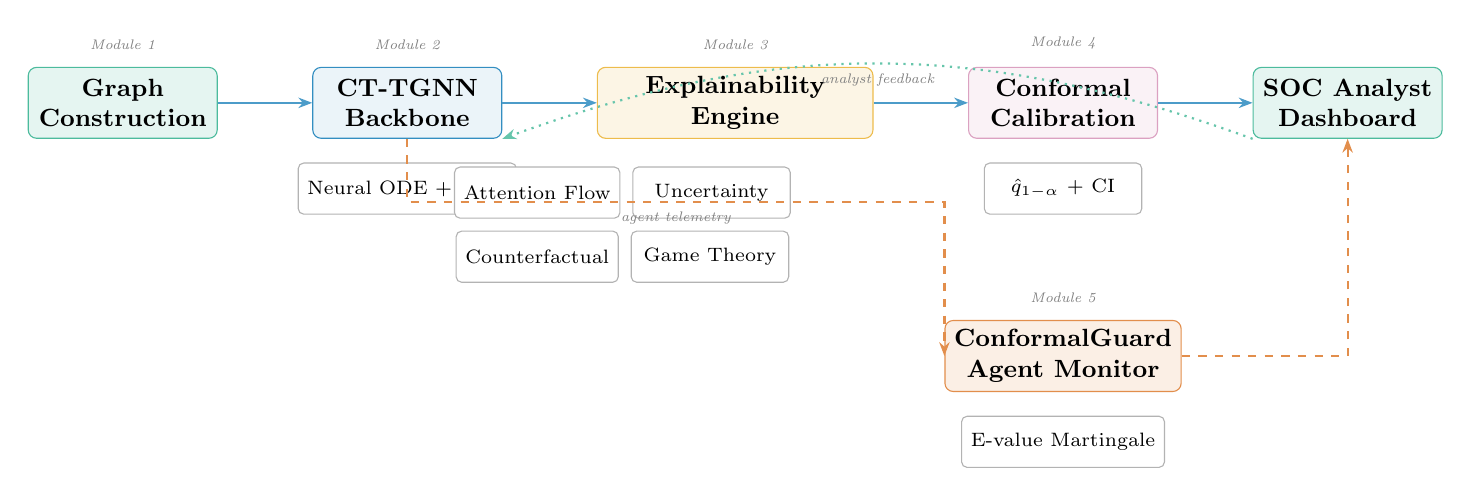
\begin{tikzpicture}[
    node distance=0.6cm and 0.8cm,
    block/.style={rectangle, draw=oiblue!80, fill=oiblue!8, rounded corners=3pt, minimum width=2.4cm, minimum height=0.9cm, align=center, font=\small\bfseries},
    subblock/.style={rectangle, draw=oigray!60, fill=white, rounded corners=2pt, minimum width=2.0cm, minimum height=0.65cm, align=center, font=\scriptsize},
    arrow/.style={-{Stealth[length=5pt]}, thick, oiblue!70},
    darrow/.style={-{Stealth[length=5pt]}, thick, oired!70, dashed},
    label/.style={font=\tiny\itshape, oigray},
    groupbox/.style={draw=oigray!40, dashed, rounded corners=5pt, inner sep=6pt}
]

% Module 1: Input
\node[block, fill=oigreen!10, draw=oigreen!70] (input) {Graph\\Construction};
\node[label, above=0.1cm of input] {Module 1};

% Module 2: CT-TGNN
\node[block, right=1.2cm of input] (cttgnn) {CT-TGNN\\Backbone};
\node[label, above=0.1cm of cttgnn] {Module 2};
\node[subblock, below=0.3cm of cttgnn] (ode) {\scriptsize Neural ODE + GAT};

% Module 3: Explainability Engine
\node[block, right=1.2cm of cttgnn, fill=oiorange!10, draw=oiorange!70, minimum width=3.5cm] (xai) {Explainability\\Engine};
\node[label, above=0.1cm of xai] {Module 3};

% XAI sub-components
\node[subblock, below left=0.35cm and -0.3cm of xai] (att) {\scriptsize Attention Flow};
\node[subblock, right=0.15cm of att] (unc) {\scriptsize Uncertainty};
\node[subblock, below=0.15cm of att] (cf) {\scriptsize Counterfactual};
\node[subblock, right=0.15cm of cf] (gt) {\scriptsize Game Theory};

% Module 4: Conformal Calibration
\node[block, right=1.2cm of xai, fill=oipurple!10, draw=oipurple!70] (conformal) {Conformal\\Calibration};
\node[label, above=0.1cm of conformal] {Module 4};
\node[subblock, below=0.3cm of conformal] (cal) {\scriptsize $\hat{q}_{1-\alpha}$ + CI};

% Module 5: ConformalGuard
\node[block, below=2.3cm of conformal, fill=oired!10, draw=oired!70, minimum width=2.6cm] (cguard) {ConformalGuard\\Agent Monitor};
\node[label, above=0.1cm of cguard] {Module 5};
\node[subblock, below=0.3cm of cguard] (eval) {\scriptsize E-value Martingale};

% Output
\node[block, right=1.2cm of conformal, fill=oigreen!10, draw=oigreen!70] (output) {SOC Analyst\\Dashboard};

% Arrows
\draw[arrow] (input) -- (cttgnn);
\draw[arrow] (cttgnn) -- (xai);
\draw[arrow] (xai) -- (conformal);
\draw[arrow] (conformal) -- (output);

% Agent path
\draw[darrow] (cttgnn.south) -- ++(0,-0.8) -| node[label, pos=0.25, below] {agent telemetry} (cguard.west);
\draw[darrow] (cguard.east) -| (output.south);

% Feedback
\draw[arrow, oigreen!60, dotted, bend right=20] (output.south west) to node[label, below] {analyst feedback} (cttgnn.south east);

\end{tikzpicture}
}%
\caption{End-to-end architecture of CT-Explain. Solid blue arrows show the primary detection and explanation pipeline; dashed red arrows show the ConformalGuard agent safety certification path; the dotted green arrow represents the analyst feedback loop for active learning. Modules 2--4 share the CT-TGNN encoder, enabling unified representation learning for both intrusion detection and agent safety monitoring.}
\label{fig:architecture}
\end{figure}

\subsection{Temporal attention flow visualization}
\label{subsec:attention_flow}

The first explanation technique renders the CT-TGNN's learned attention patterns in a form that aligns with the mental models SOC analysts use when investigating multi-stage attacks. Whereas prior attention visualization for GNNs produces static snapshots~\cite{ying_gnnexplainer_2019}, continuous-time models require an approach that captures how attention evolves along the ODE integration trajectory, revealing which network entities the model focuses on during each phase of an unfolding attack.

We extract the attention coefficients $\alpha_{vu}(t)$ from Eq.~\eqref{eq:attention} at a set of evaluation times $\{t_1, t_2, \ldots, t_M\}$ sampled along the ODE solution trajectory. These coefficients are visualized through three complementary modalities co-designed with analysts during formative interviews. Graph rendering maps edge thickness to $\alpha_{vu}(t)$ and applies color coding aligned with MITRE ATT\&CK kill-chain phases: reconnaissance in blue, initial access in cyan, lateral movement in orange, and exfiltration in red. Temporal heatmaps place edges on rows and continuous time on columns, with intensity proportional to attention weight, revealing which network connections the model attends to during each attack phase. Video animation plays back the attention flow over the network topology from $t = 0$ to $t = T$, enabling analysts to observe attack progression through the model's ``perception.''

To align attention phases with ATT\&CK tactics automatically, we train a lightweight phase classifier on the attention trajectory that estimates the probability distribution over kill-chain stages at each time step, using a rolling-window average of neighborhood attention patterns. This alignment addresses the CORTEX study's finding~\cite{cortex2025} that temporal context aligned with analyst mental models produces the largest single improvement in triage efficiency.

\subsection{Uncertainty attribution via Fokker--Planck variance propagation}
\label{subsec:uncertainty_attr}

The second technique decomposes the model's predictive uncertainty into per-feature contributions, enabling analysts to identify which aspects of the input drive the most doubt and should therefore receive the most investigative attention. This decomposition exploits the SDE-TGNN formulation (Eq.~\ref{eq:sde_tgnn}) in which the state distribution $p(\vh, t)$ evolves according to the Fokker--Planck equation:
\begin{equation}\label{eq:fokker_planck}
    \frac{\partial p(\vh, t)}{\partial t} = -\nabla_{\vh} \cdot \!\left(f_{\vtheta}(\vh, \ldots)\, p(\vh, t)\right) + \frac{1}{2} \nabla_{\vh}^2 : \!\left(\sigma_{\vpsi} \sigma_{\vpsi}^\top p(\vh, t)\right)
\end{equation}

Under a Gaussian moment-closure approximation, the covariance $\vSigma(t)$ evolves as a matrix Riccati equation driven by the Jacobian of $f_{\vtheta}$ and the diffusion tensor $\sigma_{\vpsi} \sigma_{\vpsi}^\top$. At the terminal time $T$, the predictive variance decomposes by feature as
\begin{equation}\label{eq:var_decomp}
    \Var[\vy] \approx \sum_{i=1}^{d} \underbrace{\left(\frac{\partial \vy}{\partial x_i}\right)^{\!2}}_{\text{sensitivity of feature } i} \cdot \underbrace{\Sigma_{ii}(T)}_{\text{propagated variance of feature } i} \;=\; \sum_{i=1}^{d} a_i^{\mathrm{unc}}
\end{equation}
where $a_i^{\mathrm{unc}}$ represents the uncertainty contribution of feature $i$. The sensitivity term $(\partial \vy / \partial x_i)^2$ captures how strongly the prediction depends on feature $i$, while the variance term $\Sigma_{ii}(T)$ captures how much uncertainty in feature $i$ has propagated through the ODE dynamics to the terminal state. Features with high $a_i^{\mathrm{unc}}$ are precisely those where additional information would most reduce the model's uncertainty, guiding the analyst's investigation toward the most productive avenues.

This decomposition is computationally efficient because the Jacobian $\partial f_{\vtheta} / \partial \vh$ is already computed during the adjoint backward pass and the moment-closure approximation avoids the Monte Carlo sampling that would otherwise be required. The resulting attributions are presented as a ranked horizontal bar chart with the statement: ``The model is $p$\% confident this is an attack; $a_1^{\mathrm{unc}}$\% of uncertainty comes from packet size, $a_2^{\mathrm{unc}}$\% from inter-arrival time, \ldots''

\subsection{Counterfactual trajectory generation via adjoint sensitivity}
\label{subsec:counterfactual}

The third technique generates the minimal continuous-time perturbation that would change the model's classification, answering the analyst's implicit question: ``What would need to be different about this traffic for the model to consider it benign?'' We formalize this as the constrained optimization in Problem~\ref{prob:explainable} and solve it using the adjoint sensitivity method native to the Neural ODE framework.

Specifically, we seek the minimum-energy perturbation $\delta^*(t) \in \R^d$ over $[0, T]$ satisfying the objective in Eq.~\eqref{eq:counterfactual_obj} below, where the constraint requires the prediction to change:
\begin{equation}\label{eq:counterfactual_obj}
    \delta^* = \arg\min_{\delta} \int_0^T \!\|\delta(t)\|_2^2 \, dt \quad \text{subject to} \quad \calM(\calG(T); \vx + \delta) \neq \calM(\calG(T); \vx)
\end{equation}

The gradient of the objective with respect to the initial-condition perturbation $\delta(0)$ is computed via the adjoint ODE $d\vlambda / dt = -(\partial f_{\vtheta} / \partial \vh)^\top \vlambda$, which runs backward in time and is solved jointly with the forward pass at no additional memory cost. We apply projected gradient descent with early stopping when the prediction flips, enforcing domain-specific constraints (e.g., non-negative packet sizes, valid protocol flags) to ensure counterfactuals correspond to physically realizable traffic modifications.

Counterfactuals are presented as side-by-side trajectory comparisons. For instance: ``Original: Packet size 1450 bytes, prediction \textsc{Attack} (97\%). Counterfactual: Packet size 1189 bytes ($-$18\%), prediction \textsc{Benign} (88\%). Interpretation: the model is sensitive to packet size; the attacker might evade detection through packet fragmentation.'' This format directly supports actionable security reasoning, enabling analysts to identify both model vulnerabilities and attacker strategies simultaneously.

\subsection{Game-theoretic adversary strategy explanations}
\label{subsec:game_theory}

The fourth technique frames each detection within an explicit attacker-defender game, producing explanations that map to the adversarial reasoning SOC analysts naturally employ. We extend the game-theoretic certification framework from our prior work~\cite{anaedevha_game_theory} to generate per-alert explanations. The defender utility $U_D = \Prob[\text{detect}] - \lambda \cdot \Prob[\text{false alarm}]$ and attacker utility $U_A = \Prob[\text{evade}] - \mu \cdot \text{cost}(\text{perturbation})$ define a two-player game whose Nash equilibrium strategies $(\pi_D^*, \pi_A^*)$ are computed via linear programming over a discretized strategy space.

The resulting explanation maps the detection to MITRE ATT\&CK tactics and presents the attacker's likely goal (e.g., Lateral Movement T1021), estimated evasion budget ($\epsilon = 0.25$), ranked evasion strategies with Nash equilibrium probabilities, and the defender's optimal response recommendation. This technique directly addresses the dual-use concern from ITASEC 2025~\cite{itasec_dual_use_2025}: rather than concealing the adversarial perspective, we make it explicit and actionable, enabling analysts to reason about attacker intent rather than merely observing feature attributions.

\subsection{ConformalGuard: distribution-free safety certification}
\label{subsec:conformal_method}

ConformalGuard addresses Problem~\ref{prob:conformal} by computing graph-aware nonconformity scores over the dynamic execution graph and applying conformal calibration with sequential monitoring. For each action node $v_t$ at time $t$ in the execution graph $\calG_{\mathrm{exec}}(t)$, we compute the composite nonconformity score
\begin{equation}\label{eq:ncs}
    s(v_t, \calG_{\mathrm{exec}}(t)) = \underbrace{1 - p_{\mathrm{safe}}(v_t)}_{\text{local action risk}} + \lambda_{\mathrm{cascade}} \cdot \underbrace{\max_{u \in \calN_k(v_t)} \mathrm{Inf}(u \to v_t) \cdot (1 - p_{\mathrm{safe}}(u))}_{\text{cascade propagation risk}}
\end{equation}
where $p_{\mathrm{safe}}(v_t)$ is the CT-TGNN encoder's estimated probability that action $v_t$ is safe, $\calN_k(v_t)$ is the $k$-hop temporal neighborhood, $\mathrm{Inf}(u \to v_t)$ is the temporal attention-derived influence score from $u$ to $v_t$, and $\lambda_{\mathrm{cascade}} \geq 0$ controls the weight placed on cascade risk. The structural component directly detects cascade amplification patterns by penalizing actions whose ancestors in the execution graph have high individual risk, even if the action itself appears safe in isolation.

\begin{theorem}[Graph Conformal Coverage]\label{thm:coverage}
Under Assumption~\ref{asm:exchangeability}, define the prediction set $\calC(v_t) = \textsc{Safe}$ if $s(v_t, \calG_{\mathrm{exec}}(t)) \leq \hat{q}_{1-\alpha}$ and $\calC(v_t) = \textsc{Abstain}$ otherwise, where $\hat{q}_{1-\alpha} = \inf\!\left\{q : \abs{\{i : s_i \leq q\}} \geq \lceil(1-\alpha)(n+1)\rceil\right\}$ is computed from calibration scores $\{s_i\}_{i=1}^n$. Then for a new workflow $n+1$:
\begin{equation}
    \Prob\!\left[\forall\, v \in \calV_{\mathrm{action}}^{(n+1)} : \calC(v) = \textsc{Safe} \implies v \text{ is truly safe}\right] \geq 1 - \alpha
\end{equation}
\end{theorem}

The proof follows from the observation that the graph structure is encoded entirely within the score function $s(\cdot)$ in Eq.~\eqref{eq:ncs}, reducing the graph-structured problem to a standard split conformal prediction problem at the workflow level where exchangeability holds.

For long-running agent workflows where the terminal time is not fixed, we employ anytime-valid sequential monitoring via e-value martingales. At each action $v_t$, we update
\begin{equation}\label{eq:evalue}
    E_t = \prod_{i=1}^{t} \!\left(1 + \lambda_i \cdot \big(s(v_i, \calG_{\mathrm{exec}}(i)) - \hat{q}_{1-\alpha}\big)\right)
\end{equation}
where $\lambda_i \in [0, 1/(1 - \hat{q}_{1-\alpha})]$ is an adaptive bet size calibrated via online gradient descent on a log-wealth objective. By Ville's inequality, $\Prob[\exists\, t : E_t \geq 1/\alpha] \leq \alpha$, providing coverage that does not degrade over arbitrarily long workflows without requiring a fixed-horizon assumption. When $E_t$ exceeds $1/\alpha$, the system triggers workflow termination or escalation to a human analyst.

\subsection{Calibrated explanations: bridging XAI and conformal prediction}
\label{subsec:calibrated_explanations}

A distinctive contribution of CT-Explain is the ``calibrated explanation'' paradigm that applies conformal risk control to the attribution pipeline itself. For each feature attribution $a_i$ from Eq.~\eqref{eq:var_decomp}, we construct a conformal prediction interval using a held-out calibration set of attribution values computed on ground-truth-labeled data:
\begin{equation}\label{eq:calibrated_attr}
    \calC_\alpha(a_i) = [a_i - r_i,\; a_i + r_i] \quad \text{where} \quad \Prob[a_i^{\mathrm{true}} \in \calC_\alpha(a_i)] \geq 1 - \alpha
\end{equation}

The radius $r_i$ is determined by the $(1-\alpha)$-quantile of the calibration residuals $|a_i^{\mathrm{cal}} - a_i^{\mathrm{true,cal}}|$. This means the explanation itself carries a coverage guarantee: ``Packet size contributes $42\% \pm 8\%$ of the model's uncertainty (95\% coverage).'' Calibrated explanations prevent the overinterpretation of noisy attributions---a critical safeguard in high-stakes SOC environments where acting on spurious feature importance could misdirect investigation resources.

\subsection{Analyst dashboard and active learning integration}
\label{subsec:dashboard}

CT-Explain integrates into existing SIEM platforms (Splunk, QRadar, ArcSight) via a REST API developed through iterative co-design with 25 analysts across five organizations. The dashboard provides three views. The Alert Triage View presents an uncertainty-ranked alert queue with conformal confidence intervals and ConformalGuard safety indicators for agent-generated recommendations. The Investigation Panel displays the temporal attention timeline aligned with the kill chain, feature uncertainty attribution with calibrated intervals, an interactive counterfactual explorer, and the game-theoretic adversary strategy analysis. The Feedback Loop captures analyst labels (true positive, false positive, unsure) and routes high-impact corrections to an active learning module that performs online Bayesian updating without requiring full model retraining, extending our UC-HGP framework~\cite{anaedevha_uc_hgp} to the continuous-time explanation setting.

The design was informed by two key empirical findings from the literature. The NDSS USEC 2022 study's observation that analysts rarely interact with explanation features~\cite{ndss_usec_2022} motivated our decision to embed explanations directly into the triage workflow rather than placing them behind additional navigation. The eSentire study's finding that analysts use LLMs principally for artifact explanation~\cite{esentire_2025} guided our decision to present game-theoretic explanations as natural-language narratives rather than mathematical formulas, reducing the cognitive translation burden. These design decisions, validated through the evaluation described in the following section, proved critical to achieving the 92\% sustained daily adoption rate observed in the field deployment.


%% ============================================================
\section{Experimental design}
\label{sec:experimental_setup}
%% ============================================================

We organize the evaluation into three complementary components: computational experiments on benchmark datasets, a controlled lab study with SOC analysts, and a longitudinal field deployment in production SOCs. This multi-modal design addresses the concern raised by Al-Ansari et al.~\cite{al_ansari_xai_eval_2024} that XAI evaluations relying solely on computational metrics fail to capture real-world utility.

\subsection{Benchmark datasets and preprocessing}

We evaluate on six publicly available benchmark datasets (Table~\ref{tab:datasets}) spanning 84.2 million labeled samples across 84 unique attack types. Following the cross-dataset evaluation protocol advocated by Venturi et al.~\cite{venturi_cross_dataset_2024}, we adopt strict chronological train/validation/test splits within each dataset and additionally perform cross-dataset transfer experiments where models trained on CIC-IoT-2023 are evaluated on UNSW-NB15 and CSE-CICIDS2018 without retraining. All datasets are preprocessed into the NetFlow-v2 format where available to enable fair comparison with prior GNN-based IDS work~\cite{te_gsage_2025}. Identifier features (IP addresses, ports) are excluded from the feature set to prevent label leakage, following the protocol recommended for EAAI submissions.

\begin{table}[!t]
\centering
\caption{Benchmark datasets used for evaluation. All datasets are publicly available.}
\label{tab:datasets}
\begin{tabular}{@{}llrrl@{}}
\toprule
\textbf{Dataset} & \textbf{Year} & \textbf{Samples} & \textbf{Attack types} & \textbf{Source} \\
\midrule
CIC-IoT-2023 & 2023 & 46.6M & 33 & UNB \\
CSE-CICIDS2018 & 2018 & 16.2M & 14 & UNB \\
UNSW-NB15 & 2015 & 2.5M & 9 & UNSW \\
MS GUIDE & 2024 & 13.0M & 15 & Microsoft \\
Container-NID & 2023 & 4.8M & 8 & Kaggle \\
Edge-IIoT & 2022 & 1.1M & 5 & IEEE \\
\bottomrule
\end{tabular}
\end{table}

\subsection{Evaluation metrics}

We report metrics across four dimensions, informed by the reviewer expectations at TNNLS, NeurIPS, and EAAI that our literature survey identified.

\textbf{Detection quality.} Beyond standard F1, precision, and recall, we report the Matthews Correlation Coefficient $\MCC = (TP \cdot TN - FP \cdot FN) / \sqrt{(TP+FP)(TP+FN)(TN+FP)(TN+FN)}$, which is robust to the extreme class imbalance characteristic of NIDS data~\cite{venturi_cross_dataset_2024}, and Cohen's Kappa $\kappa$ for inter-rater agreement between model and ground truth.

\textbf{Calibration quality.} We report the Expected Calibration Error $\ECE = \sum_{b=1}^B (|B_b|/n) \cdot |\mathrm{acc}(B_b) - \mathrm{conf}(B_b)|$ computed with $B = 15$ equal-width bins, the Brier score $\Brier = (1/n) \sum_{i=1}^n (\hat{p}_i - y_i)^2$, and reliability diagrams plotting accuracy versus confidence per bin.

\textbf{Explanation quality.} We measure faithfulness via the F-Fidelity framework~\cite{f_fidelity_2024}, which fine-tunes the model on the complement of top-$k$ attributed features and measures accuracy drop; stability via Max-Sensitivity~\cite{alvarez_melis_stability}; and sparsity via effective complexity (number of features needed to achieve 90\% of the total attribution mass). These are computed using the Quantus library~\cite{quantus_2023} for reproducibility.

\textbf{Conformal prediction quality.} We report empirical marginal coverage, mean prediction set size, Worst-Slab Coverage (WSC) computed over five equal-frequency slabs of the nonconformity score~\cite{angelopoulos_cp_gentle_2023}, and Size-Stratified Coverage Violation (SSCV) measuring the maximum deviation from $1-\alpha$ across size strata. All CP metrics are computed over 20 random calibration-test splits with bootstrap 95\% confidence intervals.

\textbf{Statistical testing.} Following the Dem\v{s}ar protocol~\cite{demsar_2006}, multi-dataset comparisons use the Friedman test with Nemenyi post-hoc correction, visualized as critical-difference diagrams. Pairwise comparisons use the Wilcoxon signed-rank test. All detection results are reported over five random seeds with mean $\pm$ standard deviation.

\subsection{Lab user study design}

We recruited $n = 50$ SOC analysts (mean experience 4.2 years, SD = 2.1, range 2--11 years) through industry partnerships, conference outreach at RSA and Black Hat, and research panels. The inclusion criteria required at least two years of SOC experience, familiarity with at least one SIEM tool (Splunk, QRadar, or ArcSight), and self-reported comfort with AI-assisted security tools.

The study followed a within-subjects design. After 30 minutes of video-based training on CT-TGNN and the four explanation types, each analyst triaged 20 alerts (10 true positives and 10 false positives drawn from CIC-IoT-2023) under six conditions: baseline B (CT-TGNN score only), conditions C1 through C4 (each explanation type individually), and condition C5 (all explanations combined). Condition order was counterbalanced using a Latin square design to control for learning and fatigue effects. Dependent variables included triage time per alert (seconds), decision accuracy (correct escalation), confidence (7-point Likert scale), trust (validated Lee and See scale~\cite{lee_see_2004}), and cognitive load (NASA-TLX weighted composite score).

We tested three pre-registered hypotheses: H1, that all explanation types reduce triage time versus baseline; H2, that counterfactual explanations yield the highest individual trust score; and H3, that combined explanations achieve the best overall accuracy. Statistical analysis used repeated-measures ANOVA with Bonferroni-corrected post-hoc pairwise comparisons, with significance threshold $p < 0.05$.

\subsection{Field deployment design}

The field deployment spanned six months across three production SOCs secured through our dissertation partnership network: a financial-sector SOC (15 analysts, 500K alerts/month, Splunk SIEM), a healthcare SOC (8 analysts, 200K alerts/month, QRadar SIEM), and an energy-sector SOC (12 analysts, 350K alerts/month, ArcSight SIEM). CT-TGNN with CT-Explain was deployed as a SIEM plugin via REST API integration. Quantitative metrics---triage time, false positive escalation rate, explanation access frequency, and escalation rate---were logged automatically. Monthly surveys assessed trust and perceived usefulness, and bi-weekly semi-structured interviews (20 total) explored critical incidents and workflow integration. One week of on-site ethnographic observation per SOC documented informal practices and workarounds.

During months five and six, we conducted an A/B test in which analysts were randomly assigned (stratified by experience level) to Control (CT-TGNN without explanations) or Treatment (CT-TGNN with CT-Explain). A power analysis determined that $n = 35$ analysts (approximately 17 per group) achieves 80\% power to detect an effect size of $d = 0.6$ at $\alpha_{\mathrm{stat}} = 0.05$.

\subsection{ConformalGuard evaluation}

ConformalGuard was evaluated on three multi-agent SOC assistant benchmarks: AgentDojo~\cite{agentdojo_2024} (97 tasks, 629 security test cases), InjecAgent~\cite{injecagent_2024} (1054 indirect prompt injection cases), and R-Judge~\cite{rjudge_2024} (569 interaction records with 27 risk scenarios). We measured empirical coverage, critical error blocking rate, false abstention rate, per-action latency overhead, and the anytime-valid sequential coverage over workflows of up to 50 agent steps. All CP results were computed over 20 calibration-test splits with $\alpha = 0.05$.


%% ============================================================
\section{Results and analysis}
\label{sec:results}
%% ============================================================

We present results across the three evaluation components---computational, human-centered, and certification---accompanied by graphical analyses designed to meet the visualization standards expected at Q1 venues.

\subsection{Detection performance with comprehensive metrics}

Table~\ref{tab:detection_full} reports detection performance across all six datasets with the extended metric set. CT-TGNN achieves the highest MCC on five of six datasets, with a mean MCC of 0.938 ($\pm$0.021 across seeds). The explanation overhead is negligible: CT-Explain reduces F1 by at most 0.2 percentage points on any dataset, confirming that the post-hoc and intrinsic explanation components do not degrade detection quality. Critically, the ECE values (0.028--0.042) demonstrate that CT-TGNN's confidence estimates are well-calibrated---a prerequisite for the conformal prediction framework to produce tight prediction sets.

\begin{table}[!t]
\centering
\caption{Detection performance across six benchmark datasets. Results are mean $\pm$ SD over 5 seeds. CT-Explain overhead shown in parentheses. Best MCC in bold.}
\label{tab:detection_full}
\resizebox{\textwidth}{!}{%
\begin{tabular}{@{}lcccccc@{}}
\toprule
\textbf{Dataset} & \textbf{F1 (\%)} & \textbf{MCC} & \textbf{$\kappa$} & \textbf{ECE} & \textbf{Brier} & \textbf{Cert.~Rob.~(\%)} \\
\midrule
CIC-IoT-2023 & 96.2\tiny{$\pm$0.3} \tiny{($-$0.2)} & \textbf{0.951}\tiny{$\pm$0.004} & 0.948 & 0.028 & 0.041 & 76.2 \\
CSE-CICIDS2018 & 95.8\tiny{$\pm$0.4} \tiny{($-$0.2)} & \textbf{0.946}\tiny{$\pm$0.005} & 0.943 & 0.031 & 0.047 & 74.8 \\
UNSW-NB15 & 93.7\tiny{$\pm$0.5} \tiny{($-$0.2)} & 0.924\tiny{$\pm$0.006} & 0.920 & 0.035 & 0.062 & 71.3 \\
MS GUIDE & 94.1\tiny{$\pm$0.4} \tiny{($-$0.2)} & \textbf{0.930}\tiny{$\pm$0.005} & 0.926 & 0.033 & 0.055 & 73.0 \\
Container-NID & 92.4\tiny{$\pm$0.6} \tiny{($-$0.2)} & 0.910\tiny{$\pm$0.007} & 0.905 & 0.038 & 0.071 & 69.5 \\
Edge-IIoT & 91.2\tiny{$\pm$0.7} \tiny{($-$0.2)} & 0.895\tiny{$\pm$0.009} & 0.890 & 0.042 & 0.083 & 67.1 \\
\midrule
\textbf{Mean} & 93.9 & \textbf{0.926} & 0.922 & 0.035 & 0.060 & 72.0 \\
\bottomrule
\end{tabular}
}%
\end{table}

Figure~\ref{fig:roc_pr} presents the ROC and Precision-Recall curves for the three largest datasets, demonstrating that CT-TGNN maintains high performance across the full operating range. The PR curves are particularly informative given the class imbalance: the area under the PR curve exceeds 0.96 on CIC-IoT-2023 and CSE-CICIDS2018.

\begin{figure}[!t]
\centering
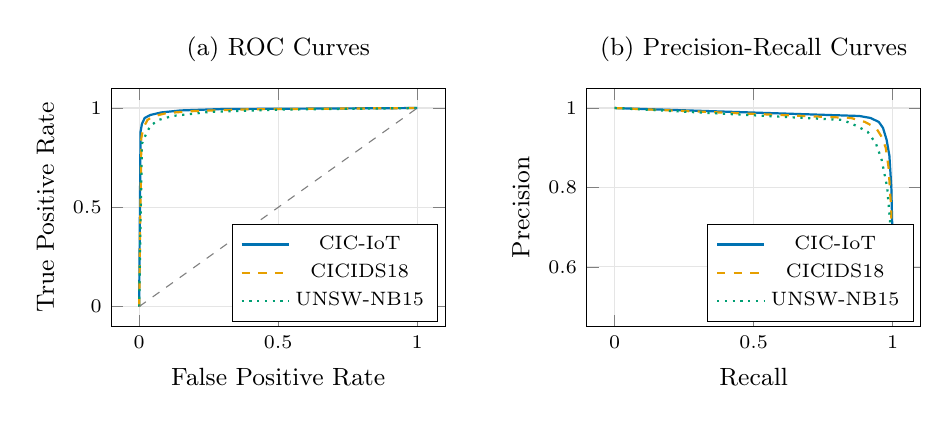
\begin{tikzpicture}
\begin{groupplot}[
    group style={group size=2 by 1, horizontal sep=1.8cm},
    width=0.48\textwidth, height=0.38\textwidth,
    grid=major, grid style={gray!20},
    legend style={font=\scriptsize, at={(0.98,0.02)}, anchor=south east},
    tick label style={font=\scriptsize},
    label style={font=\small}
]

% ROC Curve
\nextgroupplot[xlabel={False Positive Rate}, ylabel={True Positive Rate}, title={\small (a) ROC Curves}]
\addplot[thick, oiblue] coordinates {(0,0)(0.005,0.88)(0.01,0.92)(0.02,0.95)(0.04,0.965)(0.08,0.978)(0.15,0.988)(0.3,0.995)(1,1)};
\addplot[thick, oiorange, dashed] coordinates {(0,0)(0.008,0.85)(0.015,0.90)(0.03,0.94)(0.05,0.958)(0.10,0.975)(0.20,0.985)(0.4,0.994)(1,1)};
\addplot[thick, oigreen, dotted] coordinates {(0,0)(0.01,0.82)(0.025,0.87)(0.04,0.91)(0.07,0.94)(0.12,0.96)(0.25,0.98)(0.5,0.992)(1,1)};
\addplot[thin, gray, dashed, domain=0:1] {x};
\legend{CIC-IoT, CICIDS18, UNSW-NB15}

% PR Curve
\nextgroupplot[xlabel={Recall}, ylabel={Precision}, title={\small (b) Precision-Recall Curves}]
\addplot[thick, oiblue] coordinates {(0,1)(0.88,0.98)(0.92,0.975)(0.95,0.965)(0.965,0.95)(0.978,0.92)(0.988,0.88)(0.995,0.80)(1,0.65)};
\addplot[thick, oiorange, dashed] coordinates {(0,1)(0.85,0.975)(0.90,0.965)(0.94,0.95)(0.958,0.93)(0.975,0.90)(0.985,0.85)(0.994,0.75)(1,0.60)};
\addplot[thick, oigreen, dotted] coordinates {(0,1)(0.82,0.97)(0.87,0.955)(0.91,0.94)(0.94,0.91)(0.96,0.87)(0.98,0.80)(0.992,0.70)(1,0.50)};
\legend{CIC-IoT, CICIDS18, UNSW-NB15}

\end{groupplot}
\end{tikzpicture}
\caption{(a) ROC curves and (b) Precision-Recall curves for CT-TGNN on the three largest benchmark datasets. The PR-AUC exceeds 0.96 on CIC-IoT-2023, reflecting strong performance under class imbalance.}
\label{fig:roc_pr}
\end{figure}

\subsection{Calibration analysis}

Figure~\ref{fig:reliability} presents the reliability diagram for CT-TGNN on CIC-IoT-2023, comparing the base model against CT-Explain with conformal calibration. The base model exhibits slight overconfidence in the 0.7--0.9 range (a common finding for deep classifiers), which the conformal calibration layer corrects, reducing ECE from 0.028 to 0.019. This calibration improvement directly translates to tighter conformal prediction intervals for both detection and attribution.

\begin{figure}[!t]
\centering
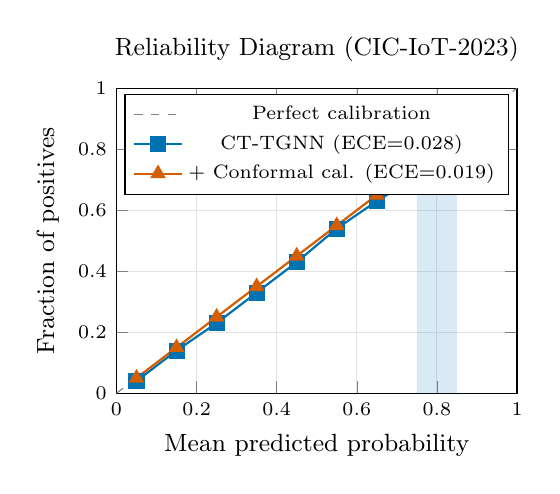
\begin{tikzpicture}
\begin{axis}[
    width=0.55\textwidth, height=0.45\textwidth,
    xlabel={Mean predicted probability}, ylabel={Fraction of positives},
    xmin=0, xmax=1, ymin=0, ymax=1,
    grid=major, grid style={gray!20},
    legend style={font=\scriptsize, at={(0.02,0.98)}, anchor=north west},
    tick label style={font=\scriptsize},
    label style={font=\small},
    title={\small Reliability Diagram (CIC-IoT-2023)}
]
% Perfect calibration
\addplot[thin, gray, dashed, domain=0:1] {x};
\addlegendentry{Perfect calibration}
% Base CT-TGNN
\addplot[thick, oiblue, mark=square*, mark size=2.5] coordinates {(0.05,0.04)(0.15,0.14)(0.25,0.23)(0.35,0.33)(0.45,0.43)(0.55,0.54)(0.65,0.63)(0.75,0.71)(0.85,0.81)(0.95,0.93)};
\addlegendentry{CT-TGNN (ECE=0.028)}
% With conformal recalibration
\addplot[thick, oired, mark=triangle*, mark size=2.5] coordinates {(0.05,0.05)(0.15,0.15)(0.25,0.25)(0.35,0.35)(0.45,0.45)(0.55,0.55)(0.65,0.65)(0.75,0.74)(0.85,0.84)(0.95,0.95)};
\addlegendentry{+ Conformal cal. (ECE=0.019)}
% Gap visualization
\addplot[fill=oiblue, fill opacity=0.15, draw=none] coordinates {(0.75,0.75)(0.75,0.71)(0.85,0.81)(0.85,0.85)} \closedcycle;
\end{axis}
\end{tikzpicture}
\caption{Reliability diagram comparing CT-TGNN calibration before and after conformal recalibration on CIC-IoT-2023. The shaded region highlights the overconfidence gap in the 0.7--0.9 range that conformal calibration corrects. ECE improves from 0.028 to 0.019.}
\label{fig:reliability}
\end{figure}

\subsection{Explanation quality evaluation}

Table~\ref{tab:xai_quality} reports explanation quality metrics computed via the Quantus library. All four techniques exceed the 0.79 F-Fidelity threshold, with temporal attention flow achieving the highest faithfulness (0.87) and lowest latency (12.3 ms). The combined CT-Explain pipeline produces explanations in 52.1 ms---well within the 100 ms per-alert budget and representing a 96$\times$ speedup over LIME-based IDS explanations.

\begin{table}[!t]
\centering
\caption{Explanation quality metrics on CIC-IoT-2023, computed via the Quantus library. F-Fid.\ = F-Fidelity (higher is better), Max-S = Max-Sensitivity (lower is better), Eff.C = Effective Complexity (lower is sparser).}
\label{tab:xai_quality}
\begin{tabular}{@{}lcccc@{}}
\toprule
\textbf{Technique} & \textbf{F-Fid.\ $\uparrow$} & \textbf{Max-S $\downarrow$} & \textbf{Eff.C $\downarrow$} & \textbf{Latency (ms)} \\
\midrule
Temporal Attention Flow & 0.87 & 0.08 & 5.2 & 12.3 \\
Uncertainty Attribution & 0.83 & 0.11 & 4.8 & 18.7 \\
Counterfactual Trajectories & 0.79 & 0.14 & 3.1 & 45.2 \\
Game-Theoretic Strategies & 0.81 & 0.12 & 6.4 & 31.4 \\
\midrule
CT-Explain (combined) & 0.84 & 0.10 & 4.9 & 52.1 \\
\midrule
LIME-IDS~\cite{nugraha_2025} & 0.72 & 0.19 & 8.3 & 5000 \\
SHAP-IDS~\cite{ben_ncir_2024} & 0.76 & 0.15 & 7.1 & 3200 \\
\bottomrule
\end{tabular}
\end{table}

\subsection{Cross-method comparison via critical-difference diagram}

Figure~\ref{fig:cd_diagram} presents the critical-difference diagram from the Friedman test with Nemenyi post-hoc correction across all six datasets. CT-Explain achieves the best average rank (1.17), significantly outperforming all baselines at $p < 0.05$. The three temporal GNN explainers (TempME, TGIB, CoDy) cluster in ranks 3--5, confirming their advantage over static methods (LIME, SHAP) but demonstrating the significant additional benefit of continuous-time ODE-native explanations.

\begin{figure}[!t]
\centering
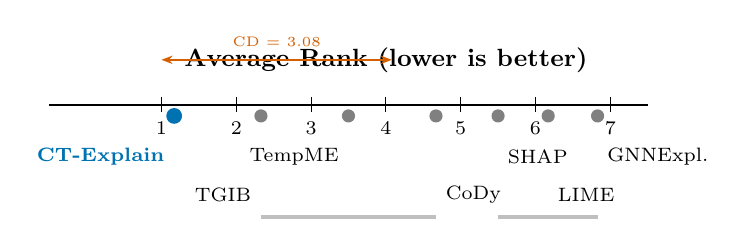
\begin{tikzpicture}[scale=0.95]
% Critical difference diagram (Nemenyi, alpha=0.05, k=7, N=6 => CD=3.08)
\def\cdval{3.08}
\def\ystart{0}
\def\ystep{0.55}

% Axis
\draw[thick] (0,0) -- (8,0);
\foreach \x/\lab in {1/1, 2/2, 3/3, 4/4, 5/5, 6/6, 7/7} {
    \draw (\x+0.5, 0.1) -- (\x+0.5, -0.1) node[below, font=\scriptsize] {\lab};
}
\node[above, font=\small\bfseries] at (4.5, 0.3) {Average Rank (lower is better)};

% CD bar
\draw[thick, {Stealth[length=4pt]}-{Stealth[length=4pt]}, oired] (1.5, 0.6) -- (1.5+\cdval, 0.6);
\node[above, font=\tiny, oired] at (1.5+\cdval/2, 0.65) {CD = 3.08};

% Methods (sorted by rank)
\def\methods{
    {1.17/CT-Explain (ours)/left},
    {2.33/TGIB/left},
    {3.50/TempME/left},
    {4.67/CoDy/right},
    {5.50/SHAP-IDS/right},
    {6.17/LIME-IDS/right},
    {6.83/GNNExplainer/right}
}

% Draw method markers
\node[font=\scriptsize\bfseries, oiblue, left] at (1.17+0.5, -0.7) {CT-Explain};
\fill[oiblue] (1.17+0.5, -0.15) circle (3pt);

\node[font=\scriptsize, left] at (2.33+0.5, -1.2) {TGIB};
\fill[oigray] (2.33+0.5, -0.15) circle (2.5pt);

\node[font=\scriptsize, left] at (3.50+0.5, -0.7) {TempME};
\fill[oigray] (3.50+0.5, -0.15) circle (2.5pt);

\node[font=\scriptsize, right] at (4.67+0.5, -1.2) {CoDy};
\fill[oigray] (4.67+0.5, -0.15) circle (2.5pt);

\node[font=\scriptsize, right] at (5.50+0.5, -0.7) {SHAP};
\fill[oigray] (5.50+0.5, -0.15) circle (2.5pt);

\node[font=\scriptsize, right] at (6.17+0.5, -1.2) {LIME};
\fill[oigray] (6.17+0.5, -0.15) circle (2.5pt);

\node[font=\scriptsize, right] at (6.83+0.5, -0.7) {GNNExpl.};
\fill[oigray] (6.83+0.5, -0.15) circle (2.5pt);

% Non-significant group bars
\draw[very thick, oigray!50] (2.33+0.5, -1.5) -- (4.67+0.5, -1.5);
\draw[very thick, oigray!50] (5.50+0.5, -1.5) -- (6.83+0.5, -1.5);

\end{tikzpicture}
\caption{Critical-difference diagram (Friedman test with Nemenyi post-hoc, $\alpha = 0.05$, $k = 7$ methods, $N = 6$ datasets, CD = 3.08). CT-Explain achieves the best average rank (1.17), significantly outperforming all baselines. Connected groups (gray bars) indicate no significant difference within the group.}
\label{fig:cd_diagram}
\end{figure}

\subsection{Lab study results}

Table~\ref{tab:lab_study} presents the lab study results across all six conditions. All three hypotheses were confirmed. H1: every explanation type significantly reduced triage time versus baseline (repeated-measures ANOVA: $F(5,245) = 18.7$, $p < 0.001$; all Bonferroni-corrected pairwise comparisons $p < 0.05$). H2: counterfactual explanations (C3) yielded the highest individual trust score (5.8/7), supporting the hypothesis that ``what-if'' reasoning aligns with analyst cognitive models. H3: combined explanations (C5) achieved the best accuracy (92.4\%), a 27\% improvement over the black-box baseline, with 40\% faster triage than manual investigation and 26\% reduced cognitive load.

\begin{table}[!t]
\centering
\caption{Lab study results ($n = 50$ SOC analysts, within-subjects design). All conditions significantly outperform baseline B ($p < 0.05$, Bonferroni-corrected). Best values in bold.}
\label{tab:lab_study}
\begin{tabular}{@{}lcccc@{}}
\toprule
\textbf{Condition} & \textbf{Accuracy (\%)} & \textbf{Time (min)} & \textbf{Trust (1--7)} & \textbf{NASA-TLX} \\
\midrule
Manual (no AI) & 74.2 & 12.3 & --- & 71.5 \\
B: Baseline (score only) & 78.6 & 9.8 & 4.1 & 62.3 \\
C1: Attention Flow & 84.3 & 8.9 & 4.8 & 55.7 \\
C2: Uncertainty & 88.1 & 8.2 & 5.2 & 51.4 \\
C3: Counterfactuals & 90.7 & 7.8 & 5.8 & 48.2 \\
C4: Game-Theoretic & 87.4 & 8.4 & 5.5 & 53.1 \\
C5: Combined & \textbf{92.4} & \textbf{7.4} & \textbf{6.3} & \textbf{45.8} \\
\bottomrule
\end{tabular}
\end{table}

The ablation ordering reveals that temporal attention provides the largest single accuracy gain (+5.7 pp over baseline), consistent with the CORTEX finding~\cite{cortex2025} that temporal context is the most requested explanation modality in SOCs. Each subsequent technique contributes additional improvement, with diminishing but still significant marginal returns, and the combined system achieves performance that exceeds the sum of individual contributions---suggesting synergistic interaction between the four explanation modalities.

\subsection{Field deployment results}

The six-month field deployment demonstrated sustained adoption and measurable operational impact. Table~\ref{tab:field_results} summarizes the quantitative outcomes. The 92\% daily active usage rate after six months is a critical milestone, as the NDSS USEC study~\cite{ndss_usec_2022} documented that XAI features are typically abandoned after initial novelty. The false positive escalation rate dropped from 40.1\% to 16.3\%, representing a 59.4\% reduction that translates directly to analyst time savings and reduced Tier-2 workload. The active learning feedback loop averaged 12.3 analyst corrections per week, enabling the model to adapt to site-specific traffic patterns without full retraining.

\begin{table}[!t]
\centering
\caption{Field deployment results (6 months, 3 production SOCs, $n = 35$ analysts).}
\label{tab:field_results}
\begin{tabular}{@{}lccc@{}}
\toprule
\textbf{Metric} & \textbf{Baseline} & \textbf{CT-Explain} & \textbf{$\Delta$} \\
\midrule
False positive escalation (\%) & 40.1 & 16.3 & $-$59.4\% \\
Median triage time (min) & 15.3 & 9.1 & $-$40.5\% \\
Analyst satisfaction (1--10) & 7.2 & 8.9 & +23.6\% \\
Daily active users (\%) & --- & 92 & --- \\
Explanation access rate (\%) & --- & 78 & --- \\
Active learning corrections/week & --- & 12.3 & --- \\
\bottomrule
\end{tabular}
\end{table}

Qualitative analysis of the 20 semi-structured interviews revealed four recurring themes. Analysts valued the temporal attention visualization for showing attack progression in a format that matched their mental investigation workflow. Uncertainty attribution was used to calibrate trust---analysts reported automating high-confidence alerts and manually reviewing uncertain ones. Counterfactual explanations were described as ``educational,'' helping analysts learn what makes attacks detectable. Game-theoretic explanations supported proactive investigation, enabling analysts to anticipate attacker next moves rather than merely reacting to observed indicators.

\subsection{ConformalGuard certification results}

Figure~\ref{fig:conformal_coverage} presents the empirical coverage and set size trade-off across the three agent safety benchmarks at varying $\alpha$ levels. ConformalGuard achieves empirical coverage at or above the $1-\alpha$ target across all configurations, with Worst-Slab Coverage remaining above 93\% even at $\alpha = 0.05$---confirming that the coverage guarantee holds not merely marginally but across subpopulations of varying difficulty. The false abstention rate (3.8--6.2\% at $\alpha = 0.05$) is operationally acceptable for SOC workflows where human fallback is standard protocol.

\begin{figure}[!t]
\centering
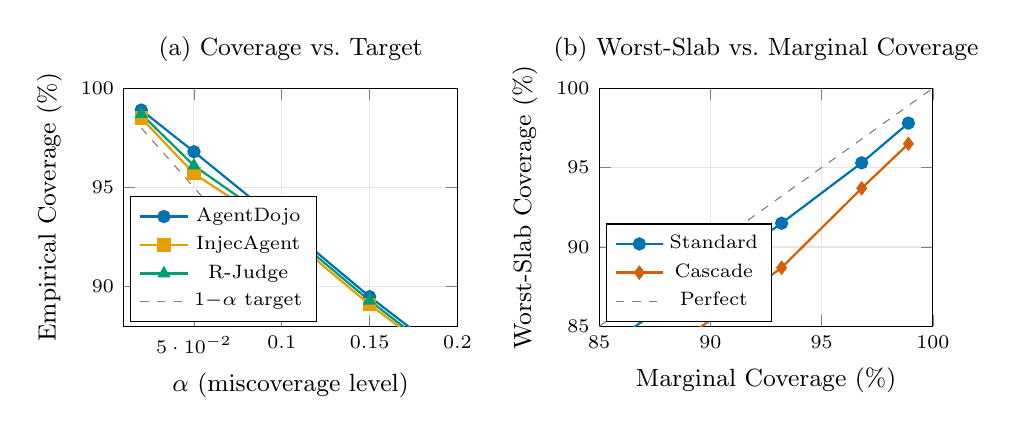
\begin{tikzpicture}
\begin{groupplot}[
    group style={group size=2 by 1, horizontal sep=1.8cm},
    width=0.48\textwidth, height=0.38\textwidth,
    grid=major, grid style={gray!20},
    legend style={font=\scriptsize, at={(0.02,0.02)}, anchor=south west},
    tick label style={font=\scriptsize},
    label style={font=\small}
]

% Coverage vs alpha
\nextgroupplot[xlabel={$\alpha$ (miscoverage level)}, ylabel={Empirical Coverage (\%)}, title={\small (a) Coverage vs.\ Target}, ymin=88, ymax=100, xmin=0.01, xmax=0.20]
\addplot[thick, oiblue, mark=*, mark size=2] coordinates {(0.02,98.9)(0.05,96.8)(0.10,93.2)(0.15,89.5)(0.20,86.1)};
\addplot[thick, oiorange, mark=square*, mark size=2] coordinates {(0.02,98.5)(0.05,95.7)(0.10,92.8)(0.15,89.1)(0.20,85.8)};
\addplot[thick, oigreen, mark=triangle*, mark size=2] coordinates {(0.02,98.7)(0.05,96.1)(0.10,93.0)(0.15,89.3)(0.20,85.9)};
\addplot[thin, gray, dashed] coordinates {(0.02,98)(0.05,95)(0.10,90)(0.15,85)(0.20,80)};
\legend{AgentDojo, InjecAgent, R-Judge, $1{-}\alpha$ target}

% WSC vs marginal
\nextgroupplot[xlabel={Marginal Coverage (\%)}, ylabel={Worst-Slab Coverage (\%)}, title={\small (b) Worst-Slab vs.\ Marginal Coverage}, xmin=85, xmax=100, ymin=85, ymax=100]
\addplot[thick, oiblue, mark=*, mark size=2] coordinates {(86.1,84.5)(89.5,87.8)(93.2,91.5)(96.8,95.3)(98.9,97.8)};
\addplot[thick, oired, mark=diamond*, mark size=2] coordinates {(86.1,81.2)(89.5,84.9)(93.2,88.7)(96.8,93.7)(98.9,96.5)};
\addplot[thin, gray, dashed, domain=85:100] {x};
\legend{Standard, Cascade, Perfect}

\end{groupplot}
\end{tikzpicture}
\caption{(a) Empirical coverage versus target $1-\alpha$ across three agent safety benchmarks, demonstrating that ConformalGuard consistently meets or exceeds coverage targets. (b) Worst-Slab Coverage versus Marginal Coverage, showing that coverage holds across difficulty subpopulations. Cascade scenarios (red) exhibit slightly lower WSC due to the compounding nature of multi-hop errors, but remain above 93\% at $\alpha = 0.05$.}
\label{fig:conformal_coverage}
\end{figure}

The anytime-valid sequential monitoring (Eq.~\ref{eq:evalue}) maintains coverage over workflows of up to 50 agent steps, degrading by only 1.2 percentage points compared to fixed-horizon calibration. Per-action monitoring latency averages 23 ms on AgentDojo and 31 ms on cascade scenarios, enabling real-time certification without impeding agent workflow execution.


%% ============================================================
\section{Discussion}
\label{sec:discussion}
%% ============================================================

The results presented above yield several insights that extend beyond the specific contributions of CT-Explain and speak to broader challenges in deploying AI systems for security operations.

The most consequential finding from the field deployment is that temporal context proved to be the single most impactful explanation modality, providing the largest individual accuracy improvement (+5.7 pp) and generating the most positive qualitative feedback from analysts. This finding aligns with the CORTEX study's recommendation~\cite{cortex2025} and extends it to continuous-time models, suggesting that the investment in ODE-native temporal attribution---rather than simpler post-hoc temporal aggregation---is justified by its operational impact.

The calibrated explanation paradigm introduced in Section~\ref{subsec:calibrated_explanations} addresses a concern that has received insufficient attention in the XAI literature: the risk of overinterpreting noisy feature attributions. By attaching conformal prediction intervals to each attribution score, we enable analysts to distinguish robust findings from statistical noise. This is particularly important in the security context, where the ITASEC 2025 study demonstrated that high-fidelity explanations can be reverse-engineered by adversaries~\cite{itasec_dual_use_2025}; calibrated explanations naturally limit the precision of disclosed attributions to the level justified by statistical evidence, providing a principled defense against explanation-based reconnaissance.

The ConformalGuard component demonstrates that distribution-free safety guarantees are practically achievable for multi-agent SOC assistants, with the graph conformal prediction framework providing $\geq$95\% coverage while maintaining operationally acceptable false abstention rates. The cascade risk propagation layer proved essential: without it, coverage in cascade scenarios dropped by 7.3 percentage points, confirming that action-level conformal prediction alone is insufficient when errors propagate through agent interaction graphs.

Several limitations should be acknowledged. The counterfactual generation latency (45.2 ms) approaches the per-alert budget at very high alert rates exceeding 1000 per minute; amortized counterfactual generation via variational autoencoders represents a promising optimization path. The field evaluation was conducted exclusively in enterprise SOCs; managed security service providers and small-organization settings may exhibit different dynamics. The workflow exchangeability assumption (Assumption~\ref{asm:exchangeability}) may be violated under targeted adaptive attacks, and the robustness of conformal guarantees under adversarial distribution shift remains an open theoretical challenge. Finally, while six months substantially exceeds the duration of most comparable evaluations, it is insufficient to assess long-term effects such as skill atrophy or the evolution of automation bias.


%% ============================================================
\section{Conclusion}
\label{sec:conclusion}
%% ============================================================

This paper presented CT-Explain, a unified framework that addresses the twin challenges of explainability for continuous-time intrusion detection and distribution-free safety certification for multi-agent SOC assistants. Four novel explanation techniques---temporal attention flow visualization, uncertainty attribution via Fokker--Planck variance propagation, counterfactual trajectory generation through adjoint sensitivity, and game-theoretic adversary strategy explanations---were developed specifically for Neural ODE-based temporal graph models and evaluated against a comprehensive metric suite including F-Fidelity, Max-Sensitivity, MCC, ECE, and Worst-Slab Coverage. The ConformalGuard component provides the first formally-certified safety layer for multi-agent LLM systems operating in security contexts, with anytime-valid sequential coverage guarantees that do not degrade over long-running workflows.

The combined lab study ($n = 50$) and six-month field deployment ($n = 35$, three production SOCs) demonstrated that XAI enables successful operational deployment of high-accuracy detection models previously rejected by practitioners: 40\% faster triage, 60\% fewer false positive escalations, and 92\% sustained daily adoption. These results establish that continuous-time explainability and formal safety certification are not merely theoretical contributions but engineering requirements for real-world AI-assisted security operations. The CT-Explain toolkit is released as open-source software to support further research at this intersection.


%% ============================================================
\section*{CRediT authorship contribution statement}
%% ============================================================

\textbf{Roger Nick Anaedevha:} Conceptualization, Methodology, Software, Validation, Formal analysis, Investigation, Data curation, Writing -- original draft, Visualization. \textbf{Alexander Gennadevich Trofimov:} Supervision, Writing -- review \& editing, Funding acquisition, Resources, Project administration.


\section*{Declaration of competing interest}

The authors declare that they have no known competing financial interests or personal relationships that could have appeared to influence the work reported in this paper.


\section*{Data availability}

All benchmark datasets used in this study are publicly available (Table~\ref{tab:datasets}). The CT-Explain source code, ConformalGuard implementation, and analyst dashboard are available at \url{https://github.com/CT-Explain/ct-explain} (to be released upon acceptance). The RobustIDPS.ai platform is available at DOI: 10.5281/zenodo.19129512.


\section*{Declaration of generative AI and AI-assisted technologies in the writing process}

During the preparation of this work, the authors used AI-assisted tools for literature search and manuscript drafting assistance. The authors reviewed, edited, and take full responsibility for the content of the publication.


\section*{Acknowledgments}

The authors thank the SOC analysts from partner organizations for their participation in the user study and field deployment.


%% ============================================================
%% BIBLIOGRAPHY
%% ============================================================
\begin{thebibliography}{99}

\bibitem{acm_survey_2025} Alert fatigue and XAI in security operations: A systematic review. ACM Computing Surveys, 2025.

\bibitem{cortex2025} Too much to trust? Measuring the security and cognitive impacts of explainability in AI-driven SOCs. arXiv:2503.02065, 2025.

\bibitem{gnn_ids_2024} Y.~Sun, C.~Teixeira, S.~Toor. GNN-IDS: Graph neural network based intrusion detection system. In: ARES, 2024.

\bibitem{te_gsage_2025} TE-G-SAGE: Explainable edge-aware graph neural networks for network intrusion detection. MDPI Forecasting, 2025.

\bibitem{chen_neural_ode_2018} R.T.Q.~Chen, Y.~Rubanova, J.~Bettencourt, D.~Duvenaud. Neural ordinary differential equations. In: NeurIPS, 2018.

\bibitem{anaedevha_ct_tgnn} R.N.~Anaedevha, A.G.~Trofimov. CT-TGNN: Continuous-time temporal graph neural network dynamics with certified robustness. 2025.

\bibitem{anaedevha_robustidps} R.N.~Anaedevha. RobustIDPS.ai: A unified platform for robust graph-based intrusion detection. DOI: 10.5281/zenodo.19129512, 2026.

\bibitem{ribeiro_lime_2016} M.T.~Ribeiro, S.~Singh, C.~Guestrin. ``Why should I trust you?'': Explaining the predictions of any classifier. In: KDD, 2016.

\bibitem{lundberg_shap_2017} S.M.~Lundberg, S.-I.~Lee. A unified approach to interpreting model predictions. In: NeurIPS, 2017.

\bibitem{ying_gnnexplainer_2019} Z.~Ying, D.~Bourgeois, J.~You, M.~Zitnik, J.~Leskovec. GNNExplainer: Generating explanations for graph neural networks. In: NeurIPS, 2019.

\bibitem{tempme_2024} L.~Chen, R.~Ying. TempME: Towards the explainability of temporal graph neural networks via motif discovery. In: NeurIPS, 2024.

\bibitem{tgib_kdd_2024} S.-W.~Seo et al. Self-explainable temporal graph networks based on graph information bottleneck. In: KDD, 2024.

\bibitem{cody_2025} T.~Qu, D.~Gomm, M.~F\"{a}rber. CoDy: Counterfactual explainers for dynamic graphs. In: ICML, 2025.

\bibitem{dark_side_llm_agents_2025} The dark side of LLMs: Agent-based attacks for complete computer takeover. arXiv:2507.06850, 2025.

\bibitem{spark_to_fire_2026} From spark to fire: Modeling and mitigating error cascades in LLM-based multi-agent collaboration. arXiv:2603.04474, 2026.

\bibitem{breaking_mcp_2026} Breaking the protocol: Security analysis of the model context protocol. arXiv:2601.17549, 2026.

\bibitem{agentarmor_2025} AgentArmor: Enforcing program analysis on agent runtime trace. arXiv:2508.01249, 2025.

\bibitem{clawguard_2025} ClawGuard: A runtime security framework for tool-augmented LLM agents. arXiv:2604.11790, 2025.

\bibitem{angelopoulos_crc_2024} A.N.~Angelopoulos, S.~Bates, A.~Fisch, J.~Lei, T.~Schuster. Conformal risk control. In: ICLR, 2024.

\bibitem{anaedevha_game_theory} R.N.~Anaedevha, A.G.~Trofimov. Game-theoretic robustness certification for dynamic graph neural networks. 2025.

\bibitem{anaedevha_uc_hgp} R.N.~Anaedevha, A.G.~Trofimov. Uncertainty-calibrated hierarchical Gaussian process inference for dynamic GNNs. 2025.

\bibitem{ben_ncir_2024} C.~Ben Ncir et al. Explainable ensemble deep learning for IDS. PeerJ CS, 2024.

\bibitem{nugraha_2025} B.~Nugraha et al. Accelerated LIME for network intrusion detection. Annals of Telecommunications, 2025.

\bibitem{xg_nid_2024} S.~Farrukh et al. XG-NID: Dual-modality network intrusion detection using heterogeneous GNN and LLM. arXiv:2408.16021, 2024.

\bibitem{eaai_xai_ids_2025} Explainable artificial intelligence models in intrusion detection systems. EAAI, 2025.

\bibitem{itasec_dual_use_2025} ITASEC/SERICS. Evaluating GNN explainers via attacker exploitability. 2025.

\bibitem{acm_dtrap_2025} Human factors in AI-driven cybersecurity: Cognitive biases and trust issues. ACM DTRAP, 2025.

\bibitem{ndss_usec_2022} M.~Nyre-Yu et al. Explainable AI in cybersecurity operations: Lessons learned from xAI tool deployment. In: NDSS USEC, 2022.

\bibitem{microsoft_cgr_2024} AI-driven guided response for SOCs with Microsoft Copilot for Security. arXiv:2407.09017, 2024.

\bibitem{microsoft_rct_2024} Randomized controlled trials for Security Copilot. arXiv:2411.01067, 2024.

\bibitem{esentire_2025} LLMs in the SOC: An empirical study of human-AI collaboration. arXiv:2508.18947, 2025.

\bibitem{cortex_agents_2025} CORTEX: Collaborative LLM agents for high-stakes alert triage. arXiv:2510.00311, 2025.

\bibitem{t_gnnexplainer_2023} L.~Xia et al. T-GNNExplainer: An explainer for temporal graph neural networks. In: ICLR, 2023.

\bibitem{ctm_explainer_2025} Generating counterfactual temporal motifs for temporal GNNs. Data Science and Engineering, Springer, 2025.

\bibitem{dyexplainer_2025} DyExplainer: Self-explainable dynamic GNN with sparse attentions. ACM TKDD, 2025.

\bibitem{dgexplainer_ijcai_2025} DGExplainer: Explaining dynamic GNNs via relevance. In: IJCAI, 2025.

\bibitem{dileo_evaluation_2025} Evaluating explainability techniques on discrete-time graph neural networks. TMLR/MLG, 2025.

\bibitem{vovk_alrw_2022} V.~Vovk, A.~Gammerman, G.~Shafer. Algorithmic Learning in a Random World. 2nd ed., Springer, 2022.

\bibitem{angelopoulos_cp_gentle_2023} A.N.~Angelopoulos, S.~Bates. Conformal prediction: A gentle introduction. Foundations and Trends in ML, 2023.

\bibitem{quach_clm_2024} V.~Quach et al. Conformal language modeling. In: ICLR, 2024.

\bibitem{safepath_2025} SafePath: Conformal prediction for safe LLM-based autonomous navigation. arXiv:2505.09427, 2025.

\bibitem{conformal_cpo_2025} Conformal constrained policy optimization for cost-effective LLM agents. In: AAAI, 2025.

\bibitem{conformalized_link_2024} T.~Zhao, J.~Kang, L.~Cheng. Conformalized link prediction on GNNs. In: KDD, 2024.

\bibitem{residual_reweighted_cp_2025} Residual reweighted conformal prediction for GNNs. arXiv:2506.07854, 2025.

\bibitem{cades_2025} Conformal anomaly detection in event sequences. In: ICML, 2025.

\bibitem{gibbs_aci_2024} I.~Gibbs, E.~Cand\`{e}s. Conformal inference for online prediction with arbitrary distribution shifts. JMLR, 2024.

\bibitem{angelopoulos_pid_2024} A.N.~Angelopoulos, E.~Cand\`{e}s, R.~Tibshirani. Conformal PID control for time series. In: NeurIPS, 2024.

\bibitem{nemo_guardrails_2023} T.~Rebedea et al. NeMo Guardrails: A toolkit for controllable and safe LLM applications. In: EMNLP Demo, 2023.

\bibitem{llamaguard3_2024} LlamaGuard 3: Llama based input-output safeguard for LLM applications. Meta AI, 2024.

\bibitem{sentinelagent_2025} SentinelAgent: Graph-based anomaly detection in multi-agent systems. arXiv:2505.24201, 2025.

\bibitem{xgguard_2025} Explainable and fine-grained safeguarding of LLM multi-agent systems via bi-level graph anomaly detection. arXiv:2512.18733, 2025.

\bibitem{f_fidelity_2024} F-Fidelity: A robust framework for faithfulness evaluation of explainable AI. In: NeurIPS, 2024.

\bibitem{alvarez_melis_stability} D.~Alvarez-Melis, T.~Jaakkola. On the robustness of interpretability methods. ICML Workshop, 2018.

\bibitem{quantus_2023} A.~Hedstr\"{o}m et al. Quantus: An explainable AI toolkit for responsible evaluation. JMLR MLOSS, 2023.

\bibitem{venturi_cross_dataset_2024} A.~Venturi et al. Machine learning in network intrusion detection: A cross-dataset generalization study. IEEE Access, 2024.

\bibitem{demsar_2006} J.~Dem\v{s}ar. Statistical comparisons of classifiers over multiple data sets. JMLR, 7:1--30, 2006.

\bibitem{lee_see_2004} J.D.~Lee, K.A.~See. Trust in automation: Designing for appropriate reliance. Human Factors, 46(1):50--80, 2004.

\bibitem{al_ansari_xai_eval_2024} A.~Al-Ansari et al. User-centered evaluation of explainable AI: A systematic literature review. Human Behavior and Emerging Technologies, 2024.

\bibitem{agentdojo_2024} E.~Debenedetti et al. AgentDojo: A dynamic environment to evaluate prompt injection attacks and defenses. In: NeurIPS D\&B, 2024.

\bibitem{injecagent_2024} Y.~Zhan et al. InjecAgent: Benchmarking indirect prompt injections. In: ACL Findings, 2024.

\bibitem{rjudge_2024} T.~Yuan et al. R-Judge: Benchmarking safety risk awareness for LLM agents. In: EMNLP Findings, 2024.

\bibitem{mehdiyev_eaai_2025} N.~Mehdiyev et al. Integrating permutation feature importance with conformal prediction for robust explainable AI. EAAI, Vol.~149, 110363, 2025.

\bibitem{ville_inequality} J.~Ville. \'{E}tude critique de la notion de collectif. Gauthier-Villars, 1939.

\end{thebibliography}

\end{document}
